\documentclass[main.tex]{subfiles}
\begin{document}
\chapter{Estado del arte}
\section[Excitones oscuros en un sistema QD-cavidad bajo un campo magnético...]{Excitones oscuros en un sistema QD-cavidad bajo un campo magnético inclinado}
El presente trabajo ``Excitones oscuros en un sistema QD-cavidad bajo un campo magnético inclinado" por \parencite{Jimenez2017} es revisado a detalle. El sistema considerado es un punto cuántico auto-ensamblado incrustado en una cavidad pilar \parencite{Kim2011}\footnote{Cabe mencionar que otras cavidades pueden ser usadas, por ejemplo, una nanocavidad cristal fotónica} bimodal,  se asume los modos polarizados a izquierda o derecha, bajo el efecto de un campo magnético con inclinación, estático y excitación coherente. La diferencia con otros trabajos \parencite{Zhang2014} es que se considera la presencia de excitones oscuros. Además, se reporta la situación donde su presencia es importante. El estudio se modela usando aproximación con la ecuación maestra, con excitación láser rápida de pulso débil. Se buscan los parámetros donde los estados excitón-oscuro se vuelven poblados y estudian la solución estacionaria para imitar los resultados experimentales. Se obtuvo que para un conjunto de parámetros es posible tener estados excitón-oscuro poblados y la presencia de los excitón-oscuro modifica fuertemente la ocupación de los modos de la cavidad. Lo cuál es adecuado para la verificación experimental

\begin{figure}[th]
	\centering
	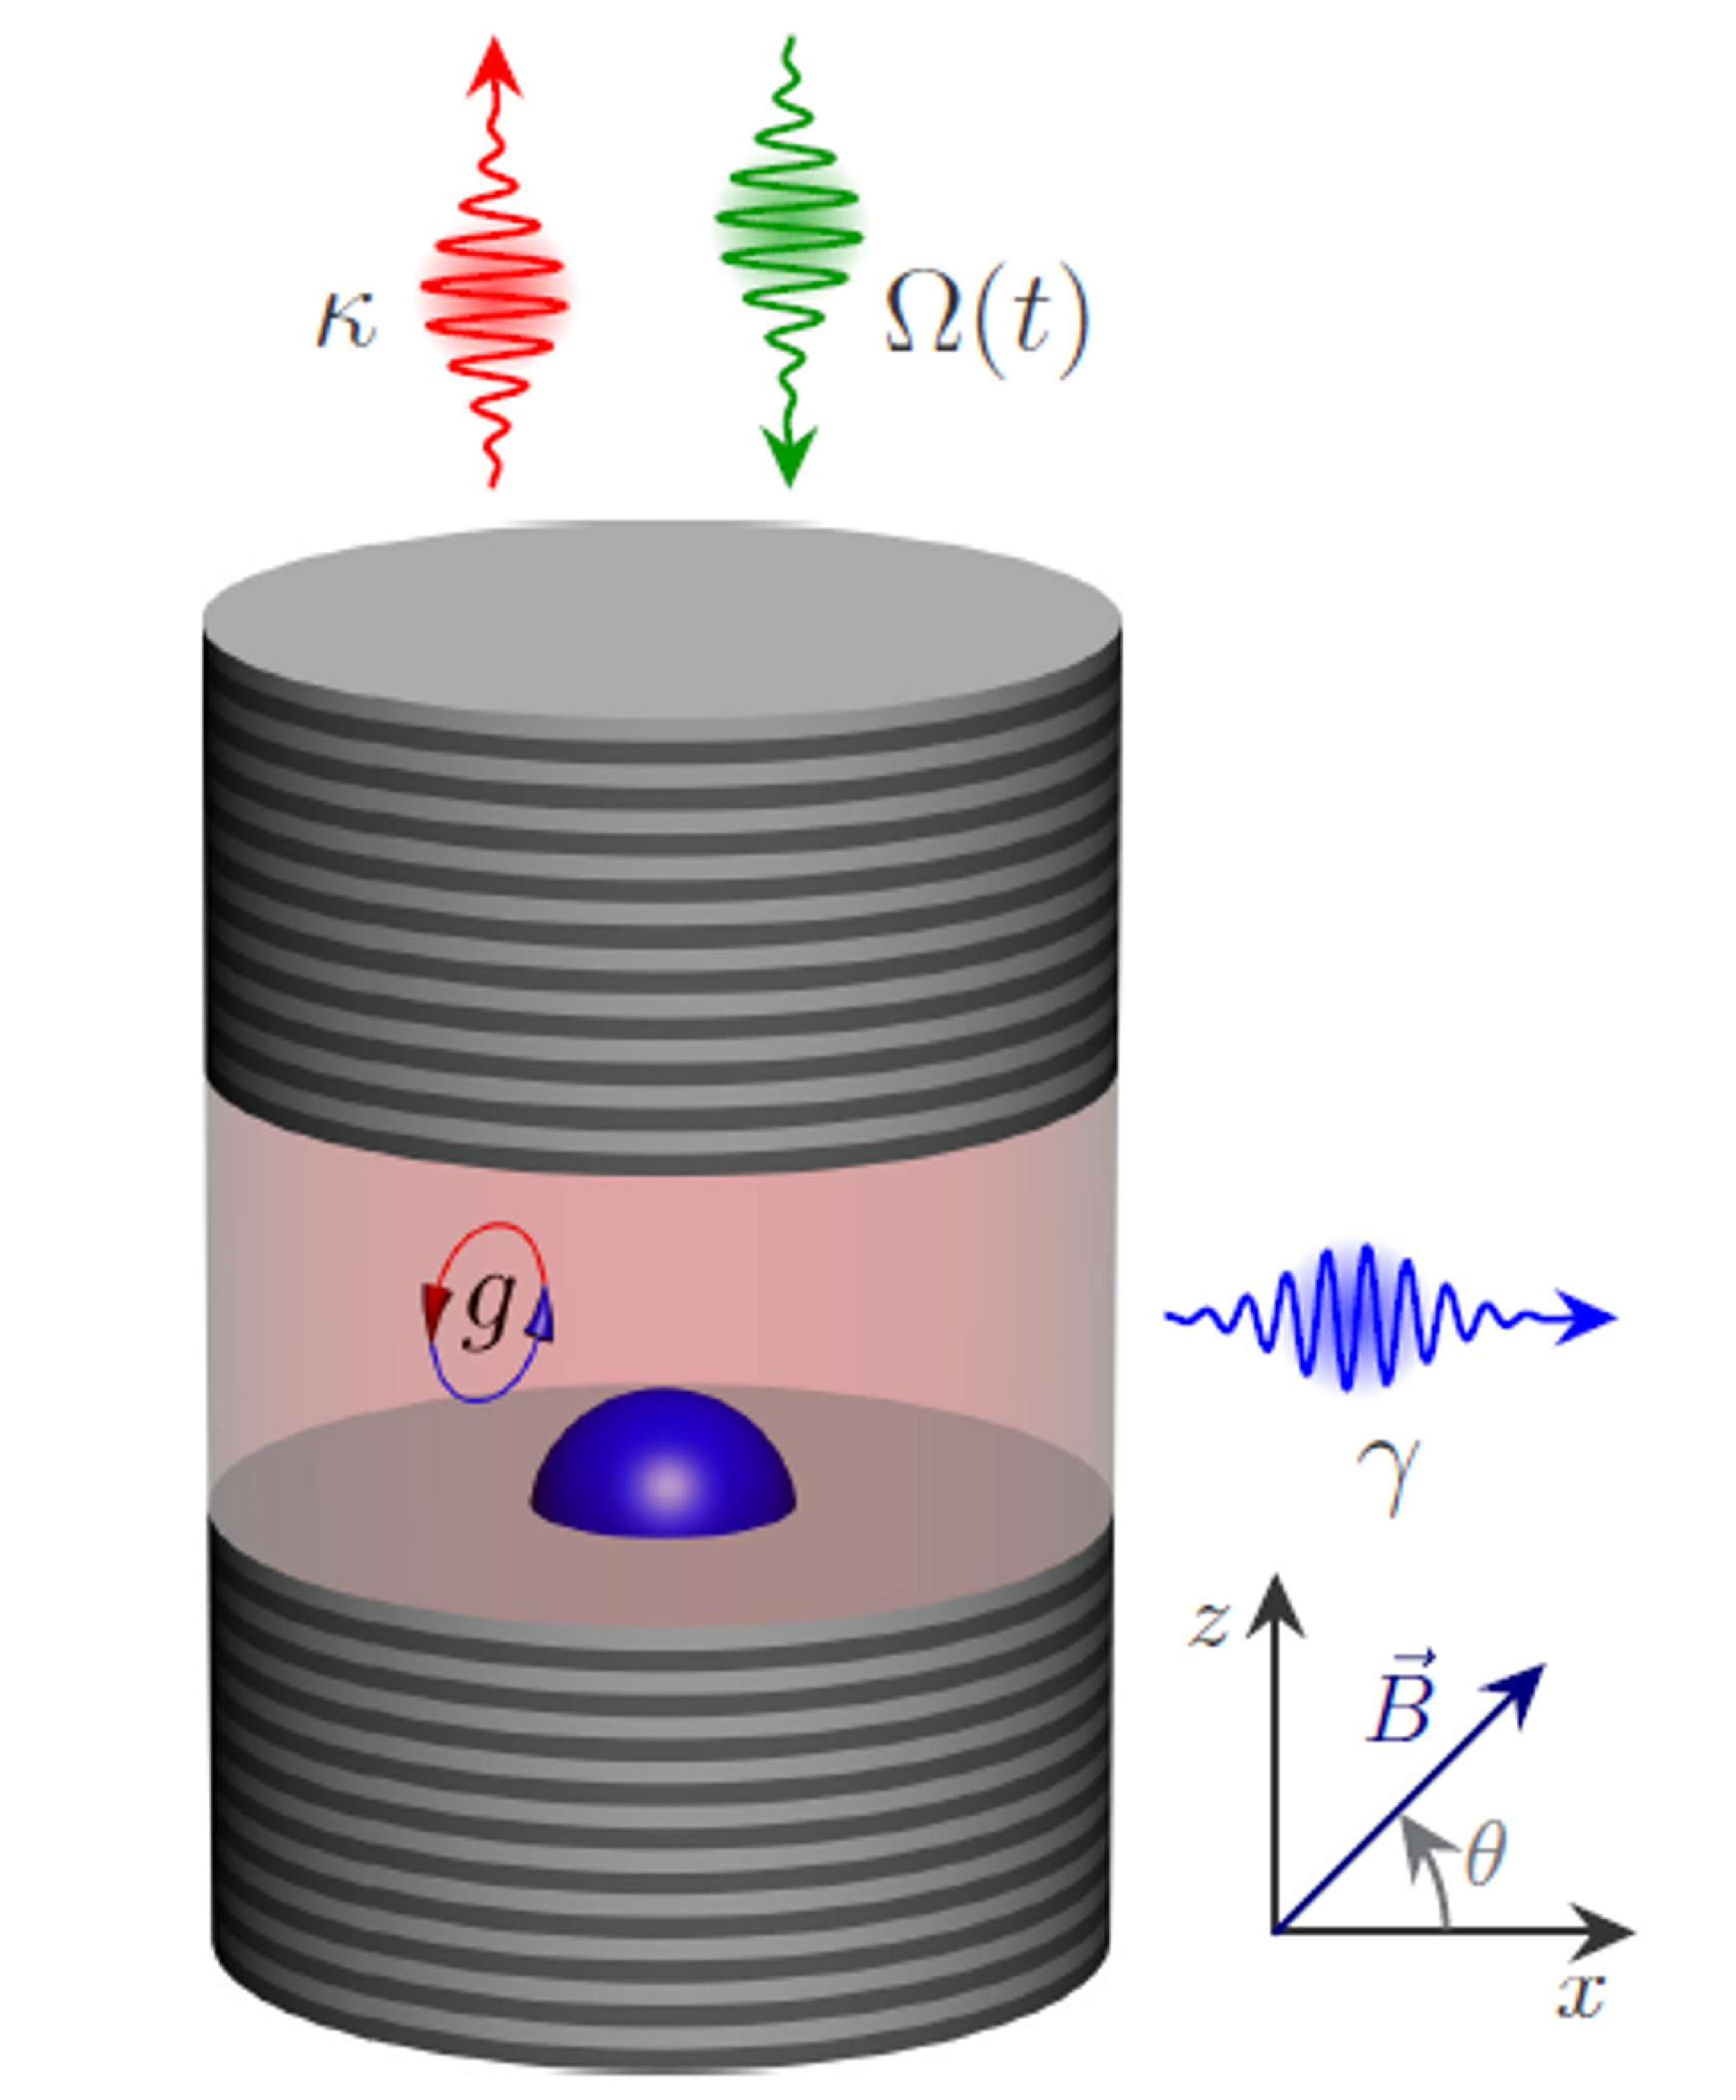
\includegraphics[width=0.35\linewidth]{img/cavidad-QD}
	\caption{Representación esquemática del sistema cavidad-QD bajo el efecto de laser pulsado $\Omega(t)$ y un campo magnético $\vec{B}$ con tasa de disipación de la cavidad $\kappa$ y tasa de decaimiento QD $\gamma$ \parencite{Jimenez2017}.}
	\label{fig:cavidad-qd}
\end{figure}

Lo característico en puntos cuánticos auto-ensamblados es la interacción de intercambio y juega un papel importante \parencite{Bayer2002}. Divide los estados excitón en brillantes y oscuros por $\delta_0$, mezcla los estados brillantes con acoplamiento $\delta_1$ conduciendo a un estado excitón brillante polarizado linealmente. Finalmente, Mezcla los estados oscuros con acoplamiento $\delta_2$ (ver fig. \ref{fig:cavidad-qdinteractions})\footnote{Se despreció estados con doble ocupación, tal como el biexcitón, debido a que se usa excitación láser de baja potencia y el efecto de fonones \parencite{Lüker2017}}

El Hamiltoniano del sistema es
\begin{equation}
	H = H_\text{QD} + H_\text{mag} + H_\text{cav} + H_\text{pump}
\end{equation}
ver ecuaciones (\ref{eq:H_QD}, \ref{eq:H_mag}, \ref{eq:H_cav}, \ref{eq:H_pump}) donde se muestra detalladamente cada uno de los términos.

\subsubsection{Análisis Hamiltoniano}

El primer estudio realizado es Hamiltoniano, es decir, primero se estudia el sistema cerrado, analizando el comportamiento de sus bandas de energía y sus estados propios variando el la intensidad del campo magnético. Suponen el acoplamiento entre excitón y cavidad independiente de su polarización, con valores $g_a = g_b = 100\text{ $\mu$eV}$. Además, se considera la tasa de decaimiento de excitón-oscuro\footnote{Eligen un valor grande para la tasa de decaimiento para mostrar que sus resultados son robustos, los valores típicos son mucho más pequeños que la tasa de decaimiento de un excitón-brillante.} $\gamma_3 = \gamma_4 = 0.1\text{$\mu$eV}$.

\begin{figure}[th]
	\centering
	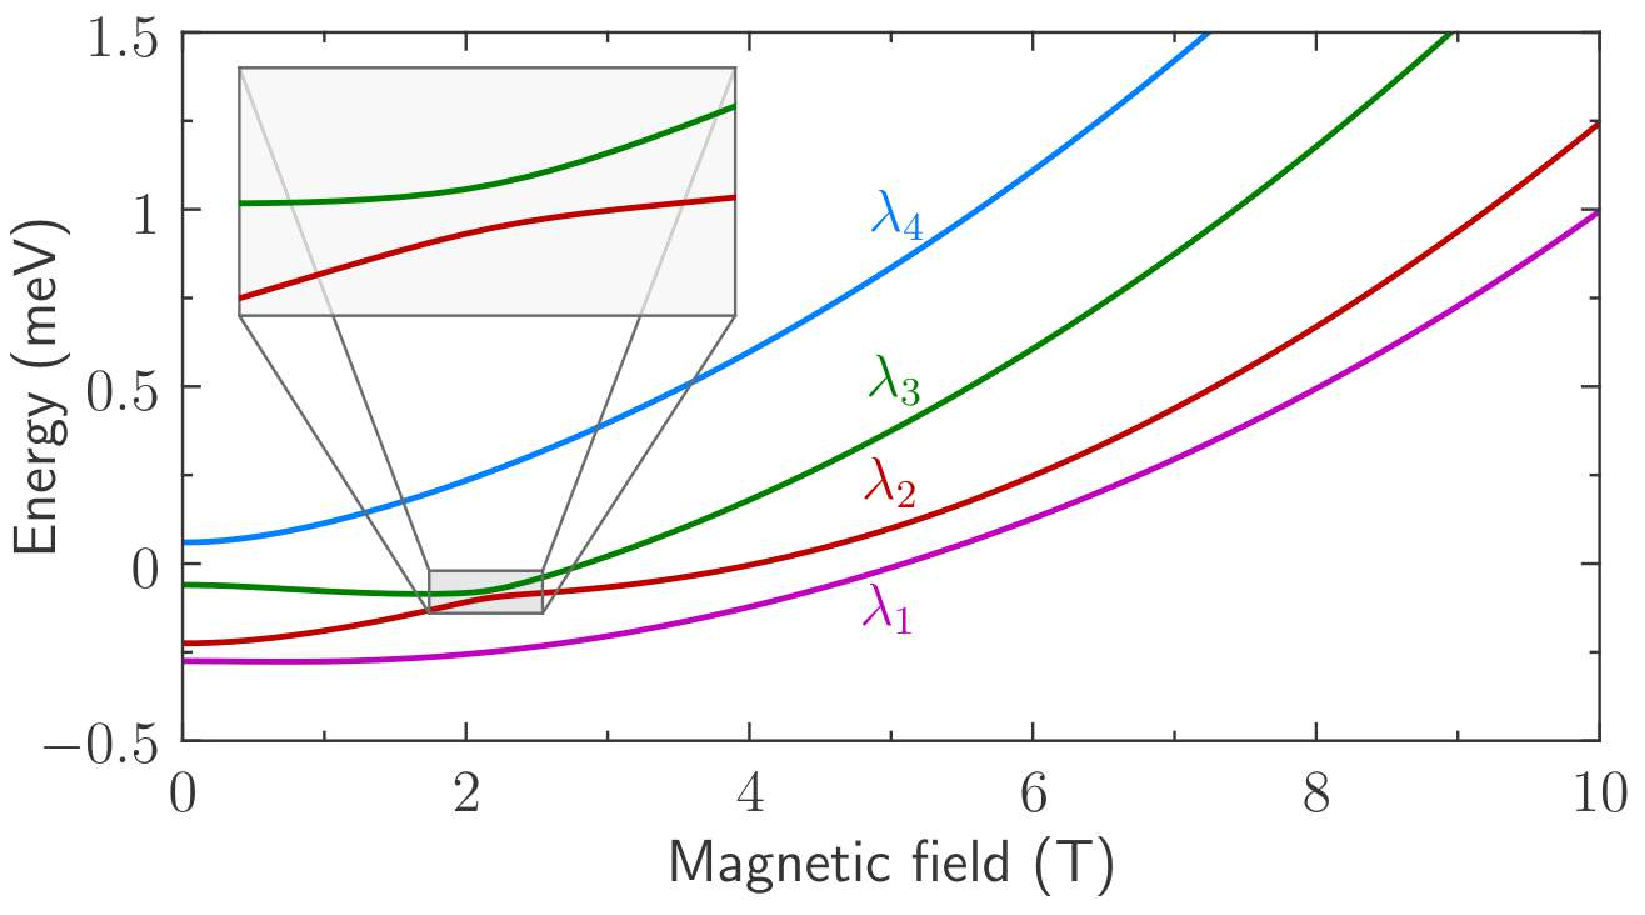
\includegraphics[width=0.6\linewidth]{img/EnergyExcitonesMagnetic}
	\caption{Espectro de energía excitónico como una función del campo magnético. Para una inclinación $\theta = \pi/3$, el recuadro muestra el anticruce \parencite{Jimenez2017}.}
	\label{fig:energyexcitonesmagnetic}
\end{figure}
Como se observa en la figura \ref{fig:energyexcitonesmagnetic} el espectro es dominado por el corrimiento diamagnético, como se esperaba.

\begin{figure}[th]
	\centering
	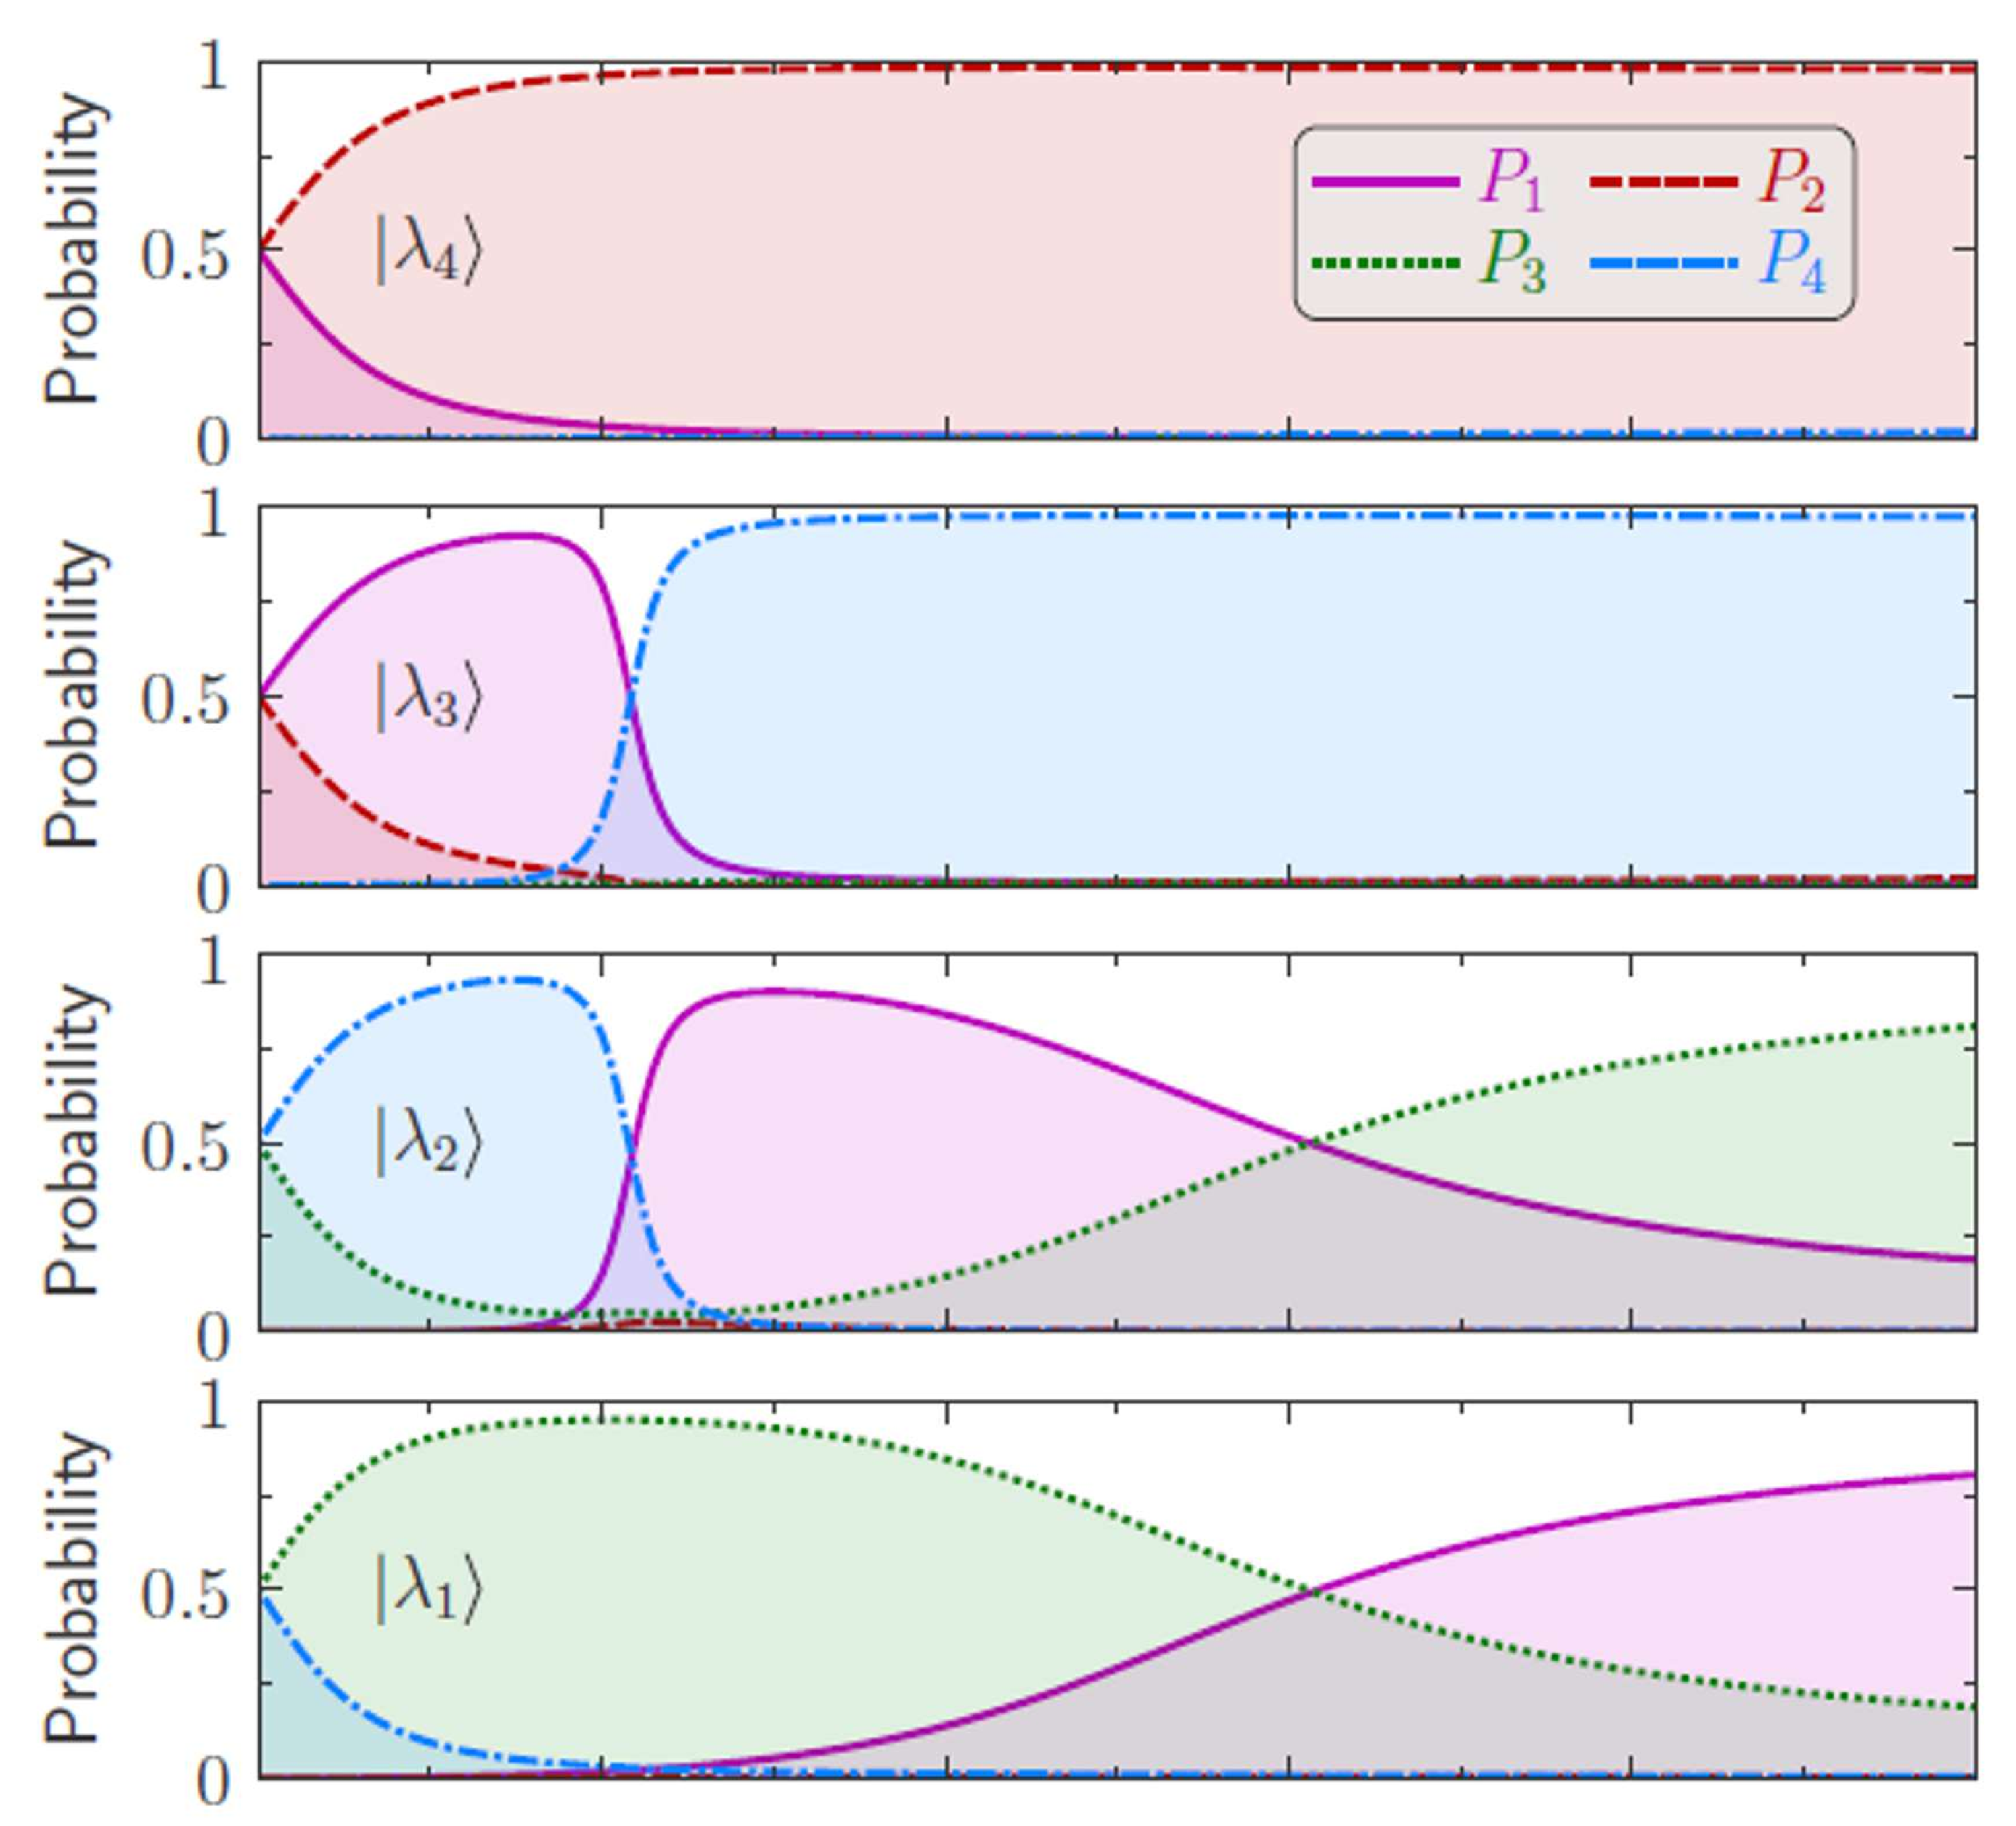
\includegraphics[width=0.7\linewidth]{img/FractionalExcitonMagnetic}
	\caption{Componentes de probabilidad de los eigenstate’s en la base excitónica desnuda (Ordenados de abajo hacia arriba con respecto a su autovalor) \parencite{Jimenez2017}.}
	\label{fig:fractionalexcitonmagnetic}
\end{figure}

De acuerdo a la figura \ref{fig:fractionalexcitonmagnetic} en $B=0$, los estados propios $\ket{\lambda_1}$ y $\ket{\lambda_2}$ son una mezcla de estados oscuros y $\ket{\lambda_3}$ y $\ket{\lambda_4}$ una mezcla de estados brillantes. Cuando se incrementa el campo magnético presenta algunos anticruces que mezcla estados excitón -oscuro y brillante. Para un campo magnético alrededor de 2 T se ve claramente la mezcla entre los estados propios $\lambda_2$ y $\lambda_3$. En 6 T se presenta otro anticruce, pero ahora entre los estados propios $\lambda_1$ y $\lambda_2$, este no se ve claramente en el espectro, pero es evidente cuando se miran las componentes de probabilidad de los estados propios correspondientes.

En campos magnéticos más altos que los mostrados la tendencia de los estados propios es convertirse en un estado excitón puro. Debido a que la división Zeeman se incrementa y supera la mezcla inicial presentada para campo magnético cero.

\subsubsection{Dinámica usando un láser pulsado}
Al estudiar la dinámica de un campo láser pulsado, en la primer búsqueda de parámetros, se puede ignorar la decoherencia\footnote{porque el bombeo es rápido $(\tau=10\text{ ps})$ y los tiempos de evolución son cortos (60 ps). Al agregar la decoherencia el único efecto observado, en los casos de prueba, fue que suavizó los valores esperados (estos resultados no son mostrados)} al evaluar los valores esperados de los estados excitón -brillante y oscuro- en un tiempo corto después del pulso (60 ps), por lo tanto, es como si se analizara la dinámica de un sistema cerrado (ver ecuaciones \ref{eq:schrodinger} y \ref{eq:neumann}) para un bombeo pulsado rápido $(\tau=10\text{ ps})$ y débil polarizado circularmente en resonancia con los modos de la cavidad $(\omega_L = \omega_a = \omega_b)$.

Eligen cuidadosamente el tamaño adecuado para la base de Fock correspondiente a cada polarización para describir correctamente el problema\footnote{Una base de Fock más pequeña que 20 estados, para cada polarización, es suficiente.}. Los resultados se muestran a continuación con gráficas de falso color que describen la probabilidad de ocupación de cada uno de los estados excitónicos en un tiempo corto después del pulso bombeado, para cada polarización, débil $\Omega_{0i}= 50\text{$\mu$eV}\; (i=a,b)$ con duración de $\tau=10\text{ ps}$ establecida en $t_c = 30\text{ ps}$:

\begin{figure}
	\centering
	
	\begin{subfigure}{0.49\textwidth}
		\centering
		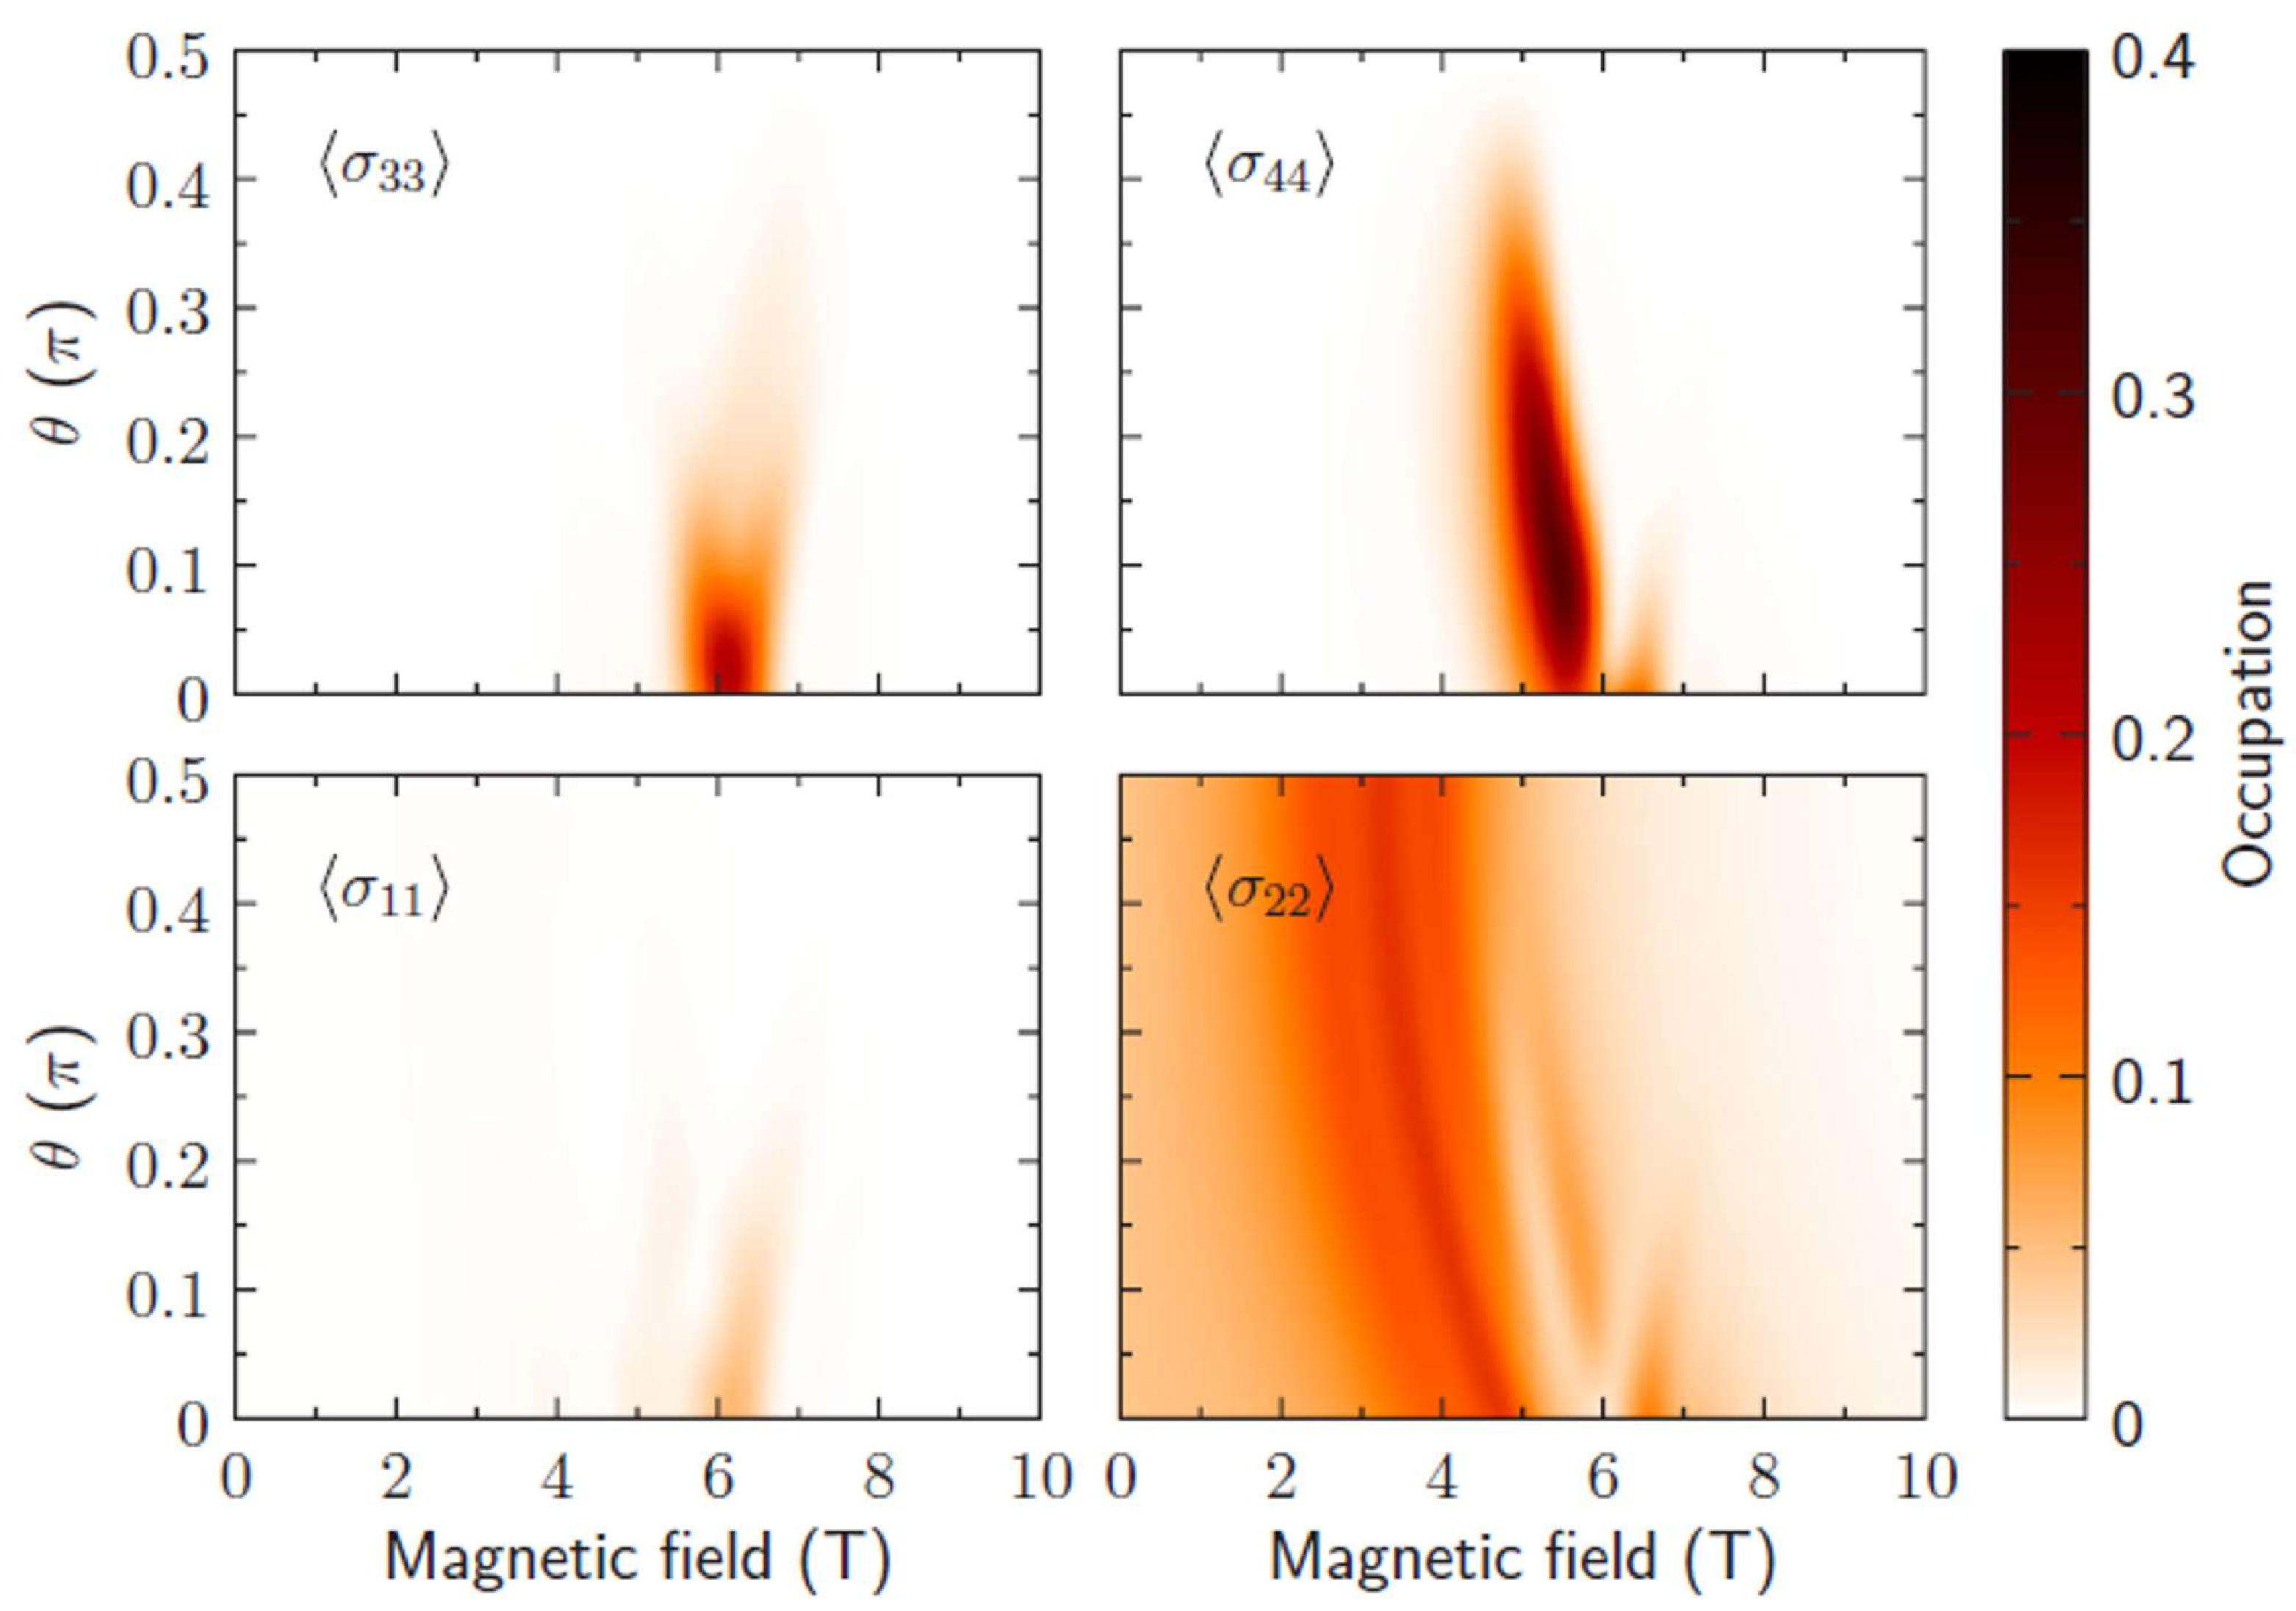
\includegraphics[width=\linewidth]{img/populationMagneticLeft}
		\caption{Polarización \textbf{izquierda}}
		\label{fig:populationmagneticleft}
	\end{subfigure}
	\hfill
	\begin{subfigure}{0.49\textwidth}
		\centering
		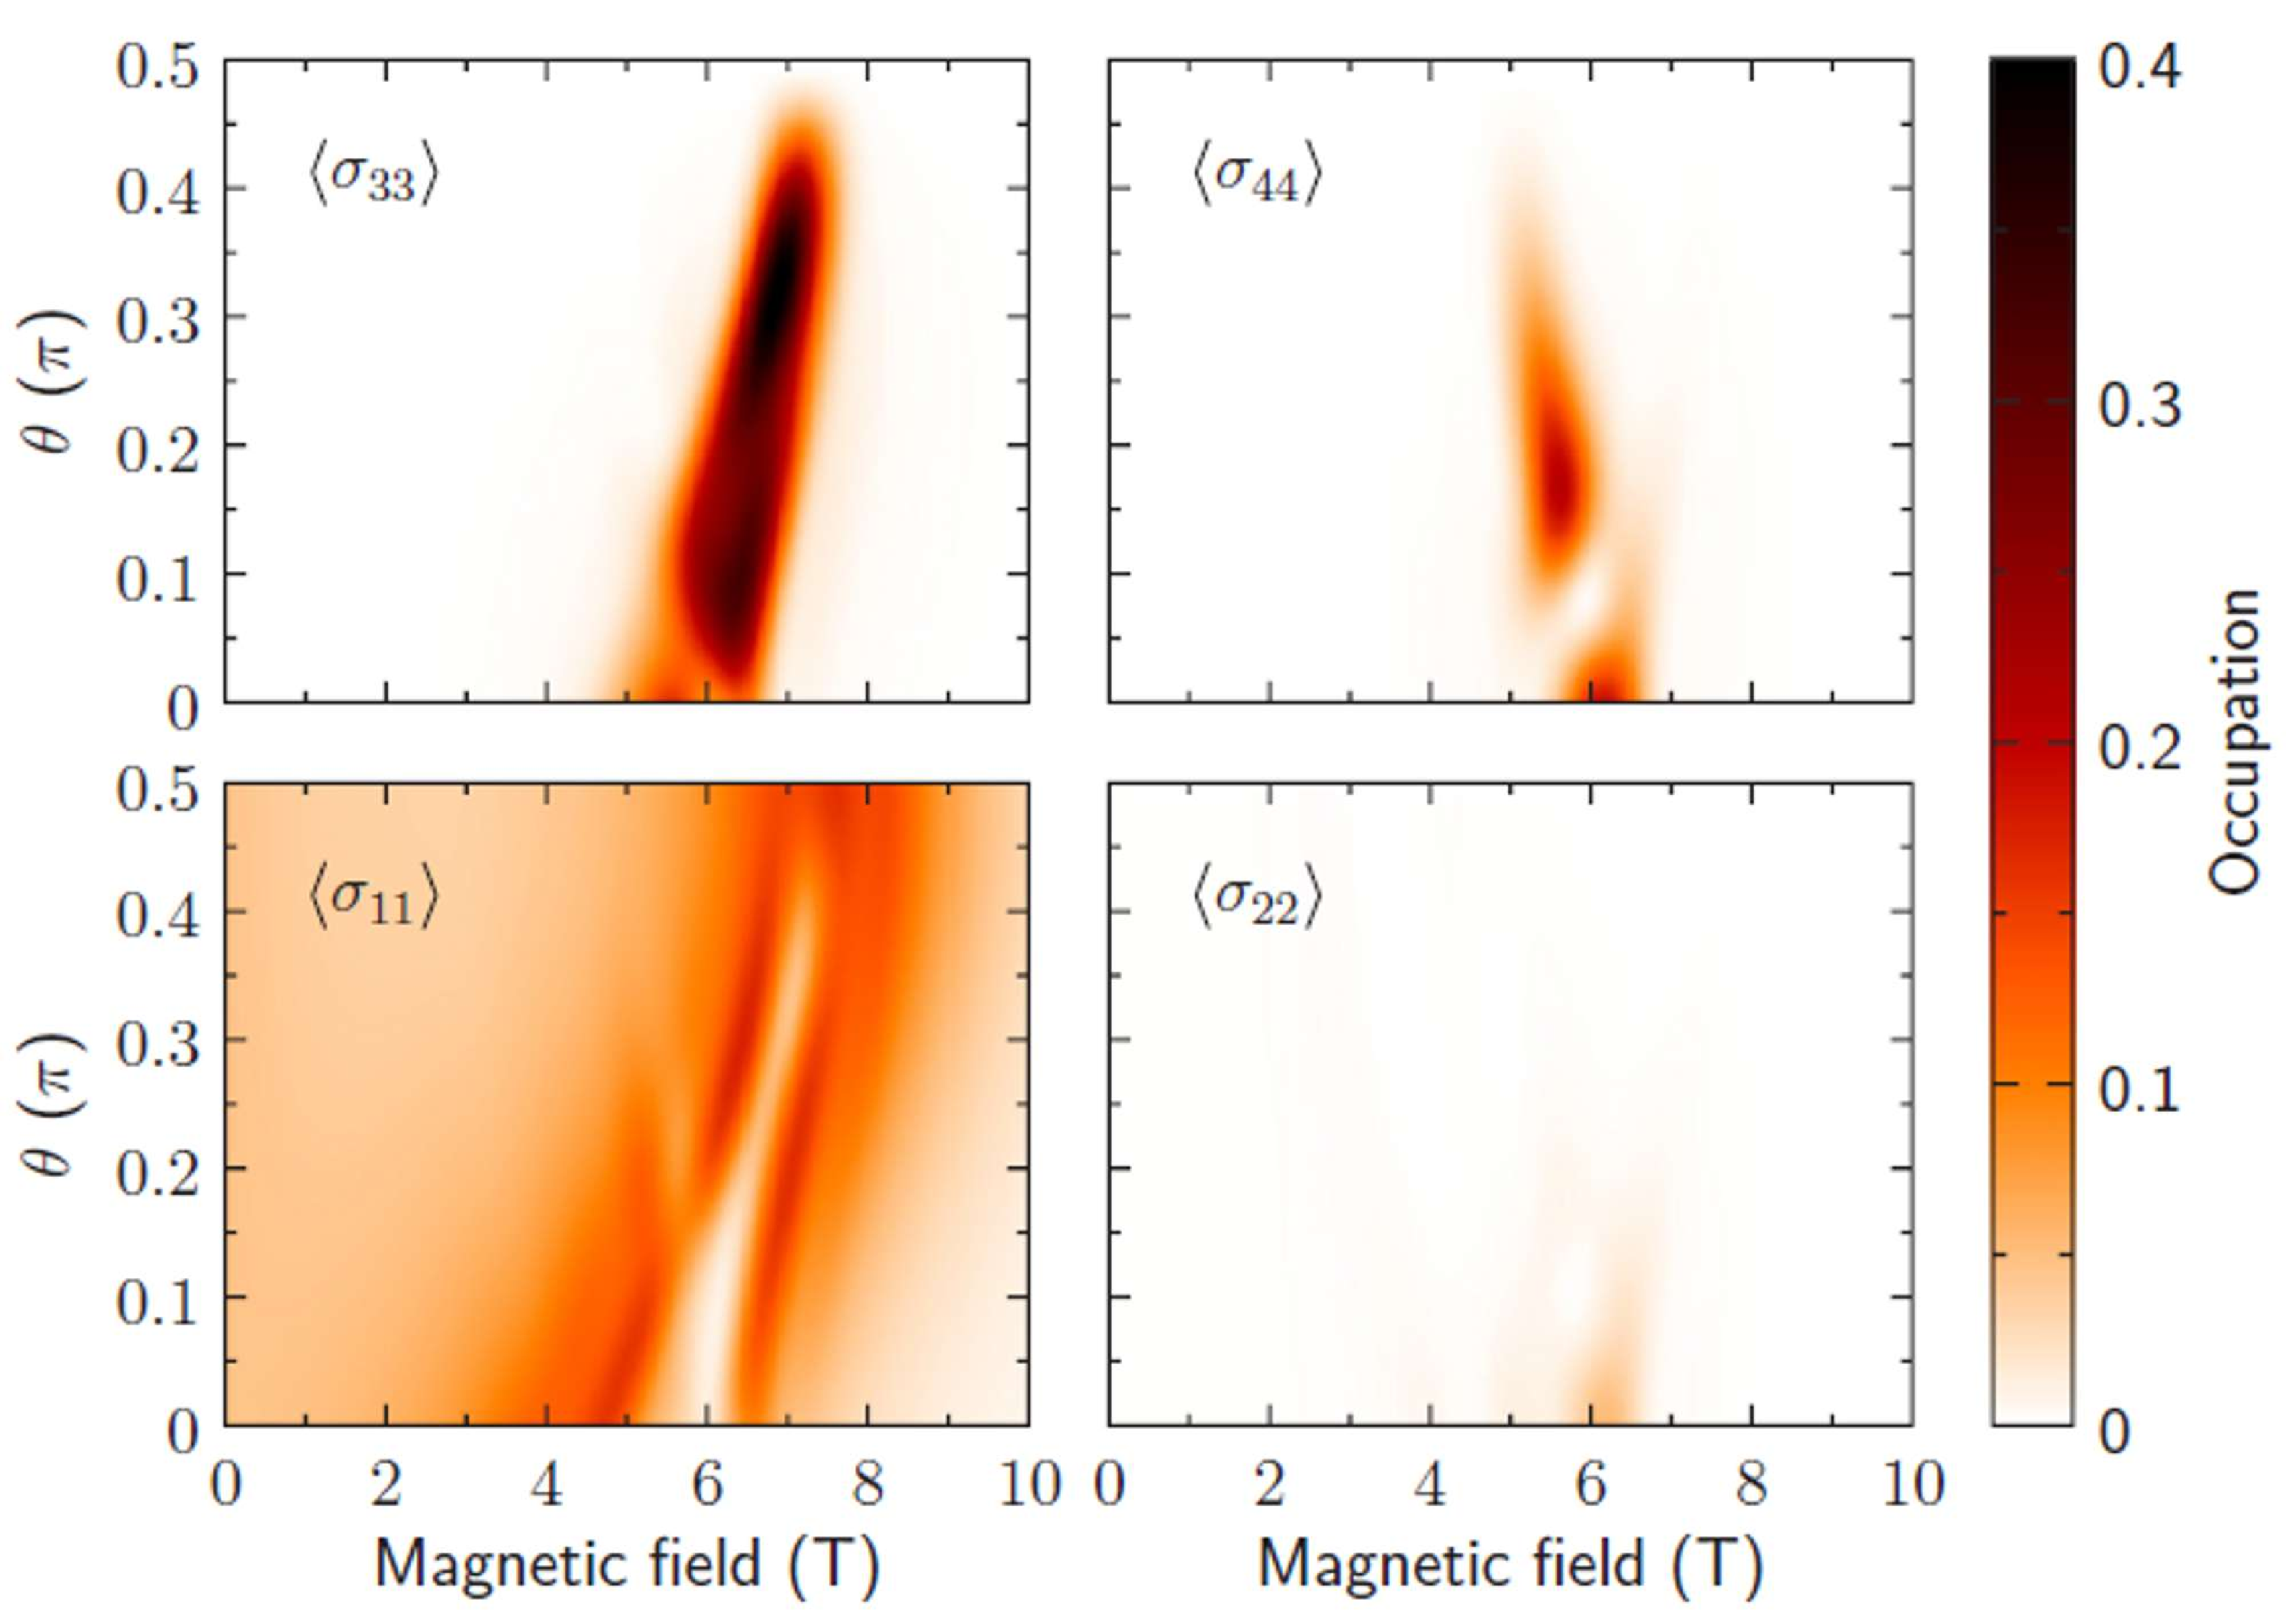
\includegraphics[width=\linewidth]{img/populationMagneticRight}
		\caption{Polarización \textbf{derecha}.}
		\label{fig:populationmagneticright}
	\end{subfigure}
	
	\caption{Dinámica de la ocupación de los estados excitónicos para un tiempo final $(t_f=60\text{ ps})$ como función del campo magnético y el ángulo de inclinación \parencite{Jimenez2017}}
	\label{fig:populationMagnetic}
\end{figure}

En la figura \ref{fig:populationmagneticright} se puede observar que ambos estados oscuros $(\braket{\sigma_{33},\, \sigma_{44}})$ pueden ser poblados. Su mejor ocupación ocurre en un campo magnético de alrededor 7 T y un ángulo del campo magnético en $\theta \simeq \pi/3$. En la figura \ref{fig:populationmagneticleft} los excitones son poblados en campos magnéticos de alrededor de 5-6 T. El ángulo en el que son más poblados es $\theta \simeq 0.1\pi$. En ambos casos se considera que los modos de la cavidad están $0.5$ meV por encima de la energía del excitón brillante,
\begin{equation}
	\omega_{a,b} = \omega_x + 0.5\text{ meV}.
\end{equation}

Concluyen que los estados oscuros no pueden ser despreciados cuando se aplique un campo magnético. Cómo se puede observar los excitones oscuros son ocupados por un rango amplio de ángulos de inclinación, incluso para la configuración de Voigt $(\theta=0)$. Excepto para la configuración de Faraday ($\theta=\pi/2$), aunque es una situación muy ideal, la cuál no representa de forma adecuada una situación experimental real, por lo que siempre se va a encontrar con una mezcla entre estados oscuros y brillantes cuando se aplica un campo magnético.

\subsubsection{Dinámica usando un campo láser continuo}

\begin{figure}[th]
	\centering
	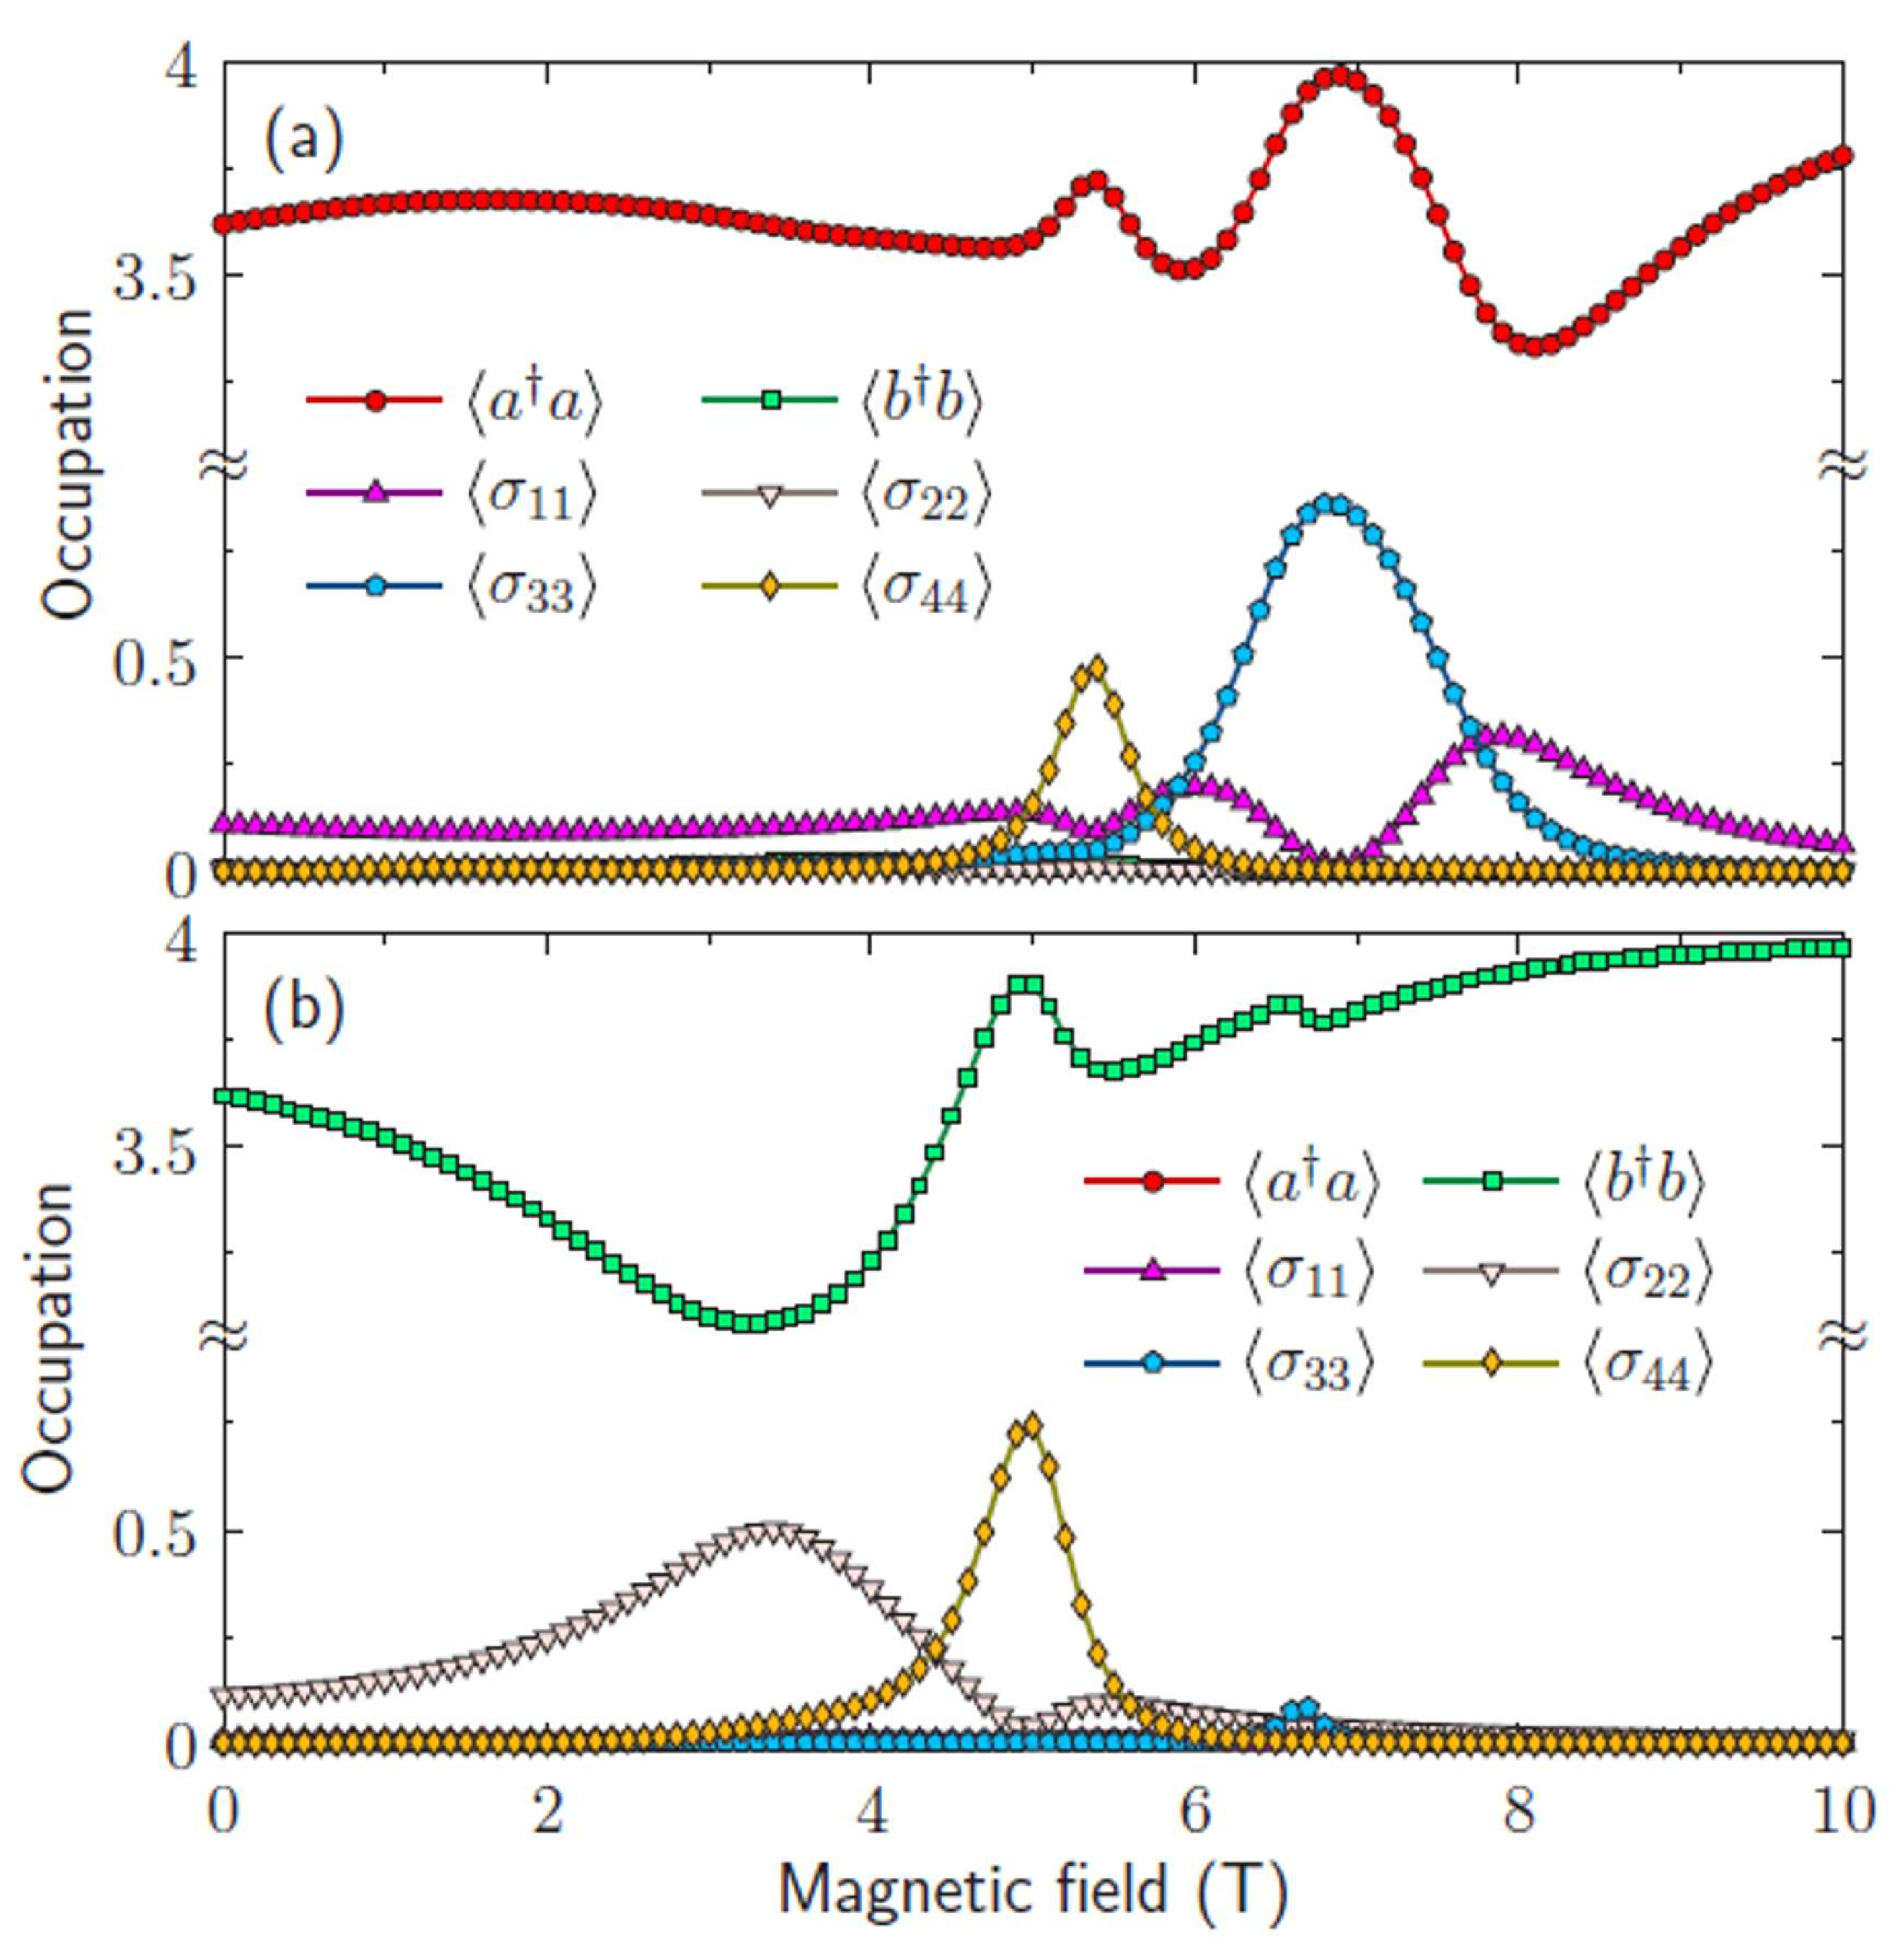
\includegraphics[width=0.7\linewidth]{img/PopulationMagnetic-cwLaser}
	\caption{Valores esperados del estado estacionario como una función de la instensidad del campo magnético. (a) Campo laser cw con polarización derecha $\Omega_a = 100\text{ $\mu$eV}$. (b) Igual que (a) para un campo láser con polarización izquierda \parencite{Jimenez2017}.}
	\label{fig:populationmagnetic-cwlaser}
\end{figure}

Al estudiar el sistema con un cw láser\footnote{Ya que en la mayoría de experimentos con QDs en cavidades en la presencia de campo magnético, se usa un bombeo láser continuo.} encuentran la situación en la que los excitones son incluso más importantes (ver figura \ref{fig:populationmagnetic-cwlaser}(a)).

Ahora se quiere encontrar la solución de estado estacionario del operador densidad\footnote{Debido a que el tiempo de integración es más largo no se puede despreciar la decoherencia}. Para ello se debe solucionar la dinámica completa (ver ec. \ref{eq:masterEquationMagnetic}). Se establecen los parámetros de simulación así: para la figura \ref{fig:populationmagnetic-cwlaser}(a) $\Omega_a = 100\text{ $\mu$eV}$, $\Omega_b = 0$, y $\theta = \pi/3$, figura \ref{fig:populationmagnetic-cwlaser}(b) $\Omega_a = 0$, $\Omega_b = 100\text{ $\mu$eV}$, y $\theta = 0.1\pi$. 

Se concluye sobre los estados de la cavidad que su ocupación estacionaria se ve fuertemente modificada cuando los estados del QD se vuelven resonantes con los modos de la cavidad, a saber, disminuye su población cuando los estados brillantes se vuelven más poblados e incrementa su población cuando los estados oscuros se vuelven más poblados. Ahora sobre los estados del QD (estados excitónicos). Cuando los estados oscuros están casi ocupados, los estados brillantes no están ocupados. Por lo tanto, para un conjunto específico de parámetros es posible poblar únicamente estados oscuros.

%conclusiones
Los excitones oscuros son muy fáciles de poblar y, por lo tanto, no pueden ser despreciados y, como se puede observar en todos los casos, la presencia de estados oscuros modifica fuertemente la ocupación del modo de la cavidad, haciendo esta consideración muy importante para el entendimiento de un sistema QD en una cavidad bajo el efecto del campo magnético.

\section{Emisión bundle de $N$-fonones por medio del proceso de Stokes}\label{sec:StokesBundles}

En este artículo \parencite{Bin2020} presentan un método para implementar la emisión de $n$-fonones bundle de un punto cuántico (QD) acoplado a una nanocavidad acústica con acoplamiento electrón-fonón e impulsado coherentemente por un láser en la banda lateral de los fonones de $n$-ésimo orden. Este proceso de Stokes impulsado ópticamente realiza oscilaciones gigante-Rabi \parencite{Strekalov2014} entre estados con gran diferencia en su número de excitaciones. La emisión pura del bundle puede lograrse abriendo un canal disipasivo para tales oscilaciones gigante-Rabi inducidas por las resonancias de Stokes. Se tiene un mecanismo físico para lograr oscilaciones gigante-Rabi, por ejemplo, a través del proceso de Stokes impulsado ópticamente. En particular, el giro del QD es acompañado por una generación de $n$-fonones en la cavidad, inducido por la interacción electrón-fonón.

El trabajo introduce los procesos de Stokes dentro de la teoría de emisión Bundle. Este régimen ampliado junto con la estructura de niveles más compleja muestra que la emisión bundle de $n$-cuantos no es limitado a plataformas y configuraciones particulares, sino que puede ser explotado en configuraciones más generales\footnote{En particular, ya que la resonancia de Stokes ideal se puede realizar sobre un amplio rango de parámetros.}. Este mecanismo conlleva a una serie de ventajas exclusivas que presenta nuestra propuesta, por ejemplo, la implementación es robusta al variar las intensidades de acoplamiento electrón-fonón y/o las intensidades de impulso, que únicamente cambia las condiciones resonantes. Esto deja mucho margen para lograr la emisión del bundle de $n$-fonones y optimizar su pureza, las actuales cifras de mérito \parencite{Stock2011} se encuentran cerca de un 99\% de emisión de dos-fonones y 97\% de emisión de tres-fonones. Además, aquí se tiene la emisión mezclada fonón-fotón, lo cual nos permite aislar eficiente y convenientemente la útil emisión de $n$-fonones de los otros (ópticos) canales de desexcitación. El modelo se podría usar para la realización de láseres y cañones de $n$-fonones anunciados ópticamente.

La propuesta abre aplicaciones potenciales para las comunicaciones cuánticas en chips, por ejemplo, la transferencia de información cuántica con bundles de fonones en futuras redes cuánticas en chip \parencite{Bienfait2019}.

Un modelo a considerar donde se tengan resonancias de Stokes es en cQED\footnote{Electrodinámica cuántica de cavidades} fonónica con un QD, de dos niveles\footnote{estado banda de conducción $\ket{c}$ y estado banda de valencia $\ket{v}$}, acoplado a un modo monofonónico de una nanocavidad acústica con acoplamiento electrón-fonon e impulsado por un láser óptico. Por lo tanto, el Hamiltoniano del sistema es
\begin{equation}
	H = H_\text{cav-ph} + H_\text{2-QD} + H_\text{2-el-ph} + H_\text{2-láser}
\end{equation}

\subsubsection{Dinámica del sistema cerrado}
Los autores hacen el análisis del sistema cerrado (ver ecs. \ref{eq:schrodinger} y \ref{eq:neumann}) en tres regímenes de resonancias de Stokes (ver sección \ref{sec:resonancesStokes}) para encontrar las oscilaciones esencialmente perfectas gigante-Rabi $\ket{0,v} \leftrightarrow \ket{n,c}$, $\ket{0,v} \leftrightarrow \ket{\tilde{n},c}$ y $\ket{0,+} \leftrightarrow \ket{n,-}$, en la ausencia de disipación (ver fig. \ref{fig:super-rabi}).

\begin{figure}[th]
	\centering
	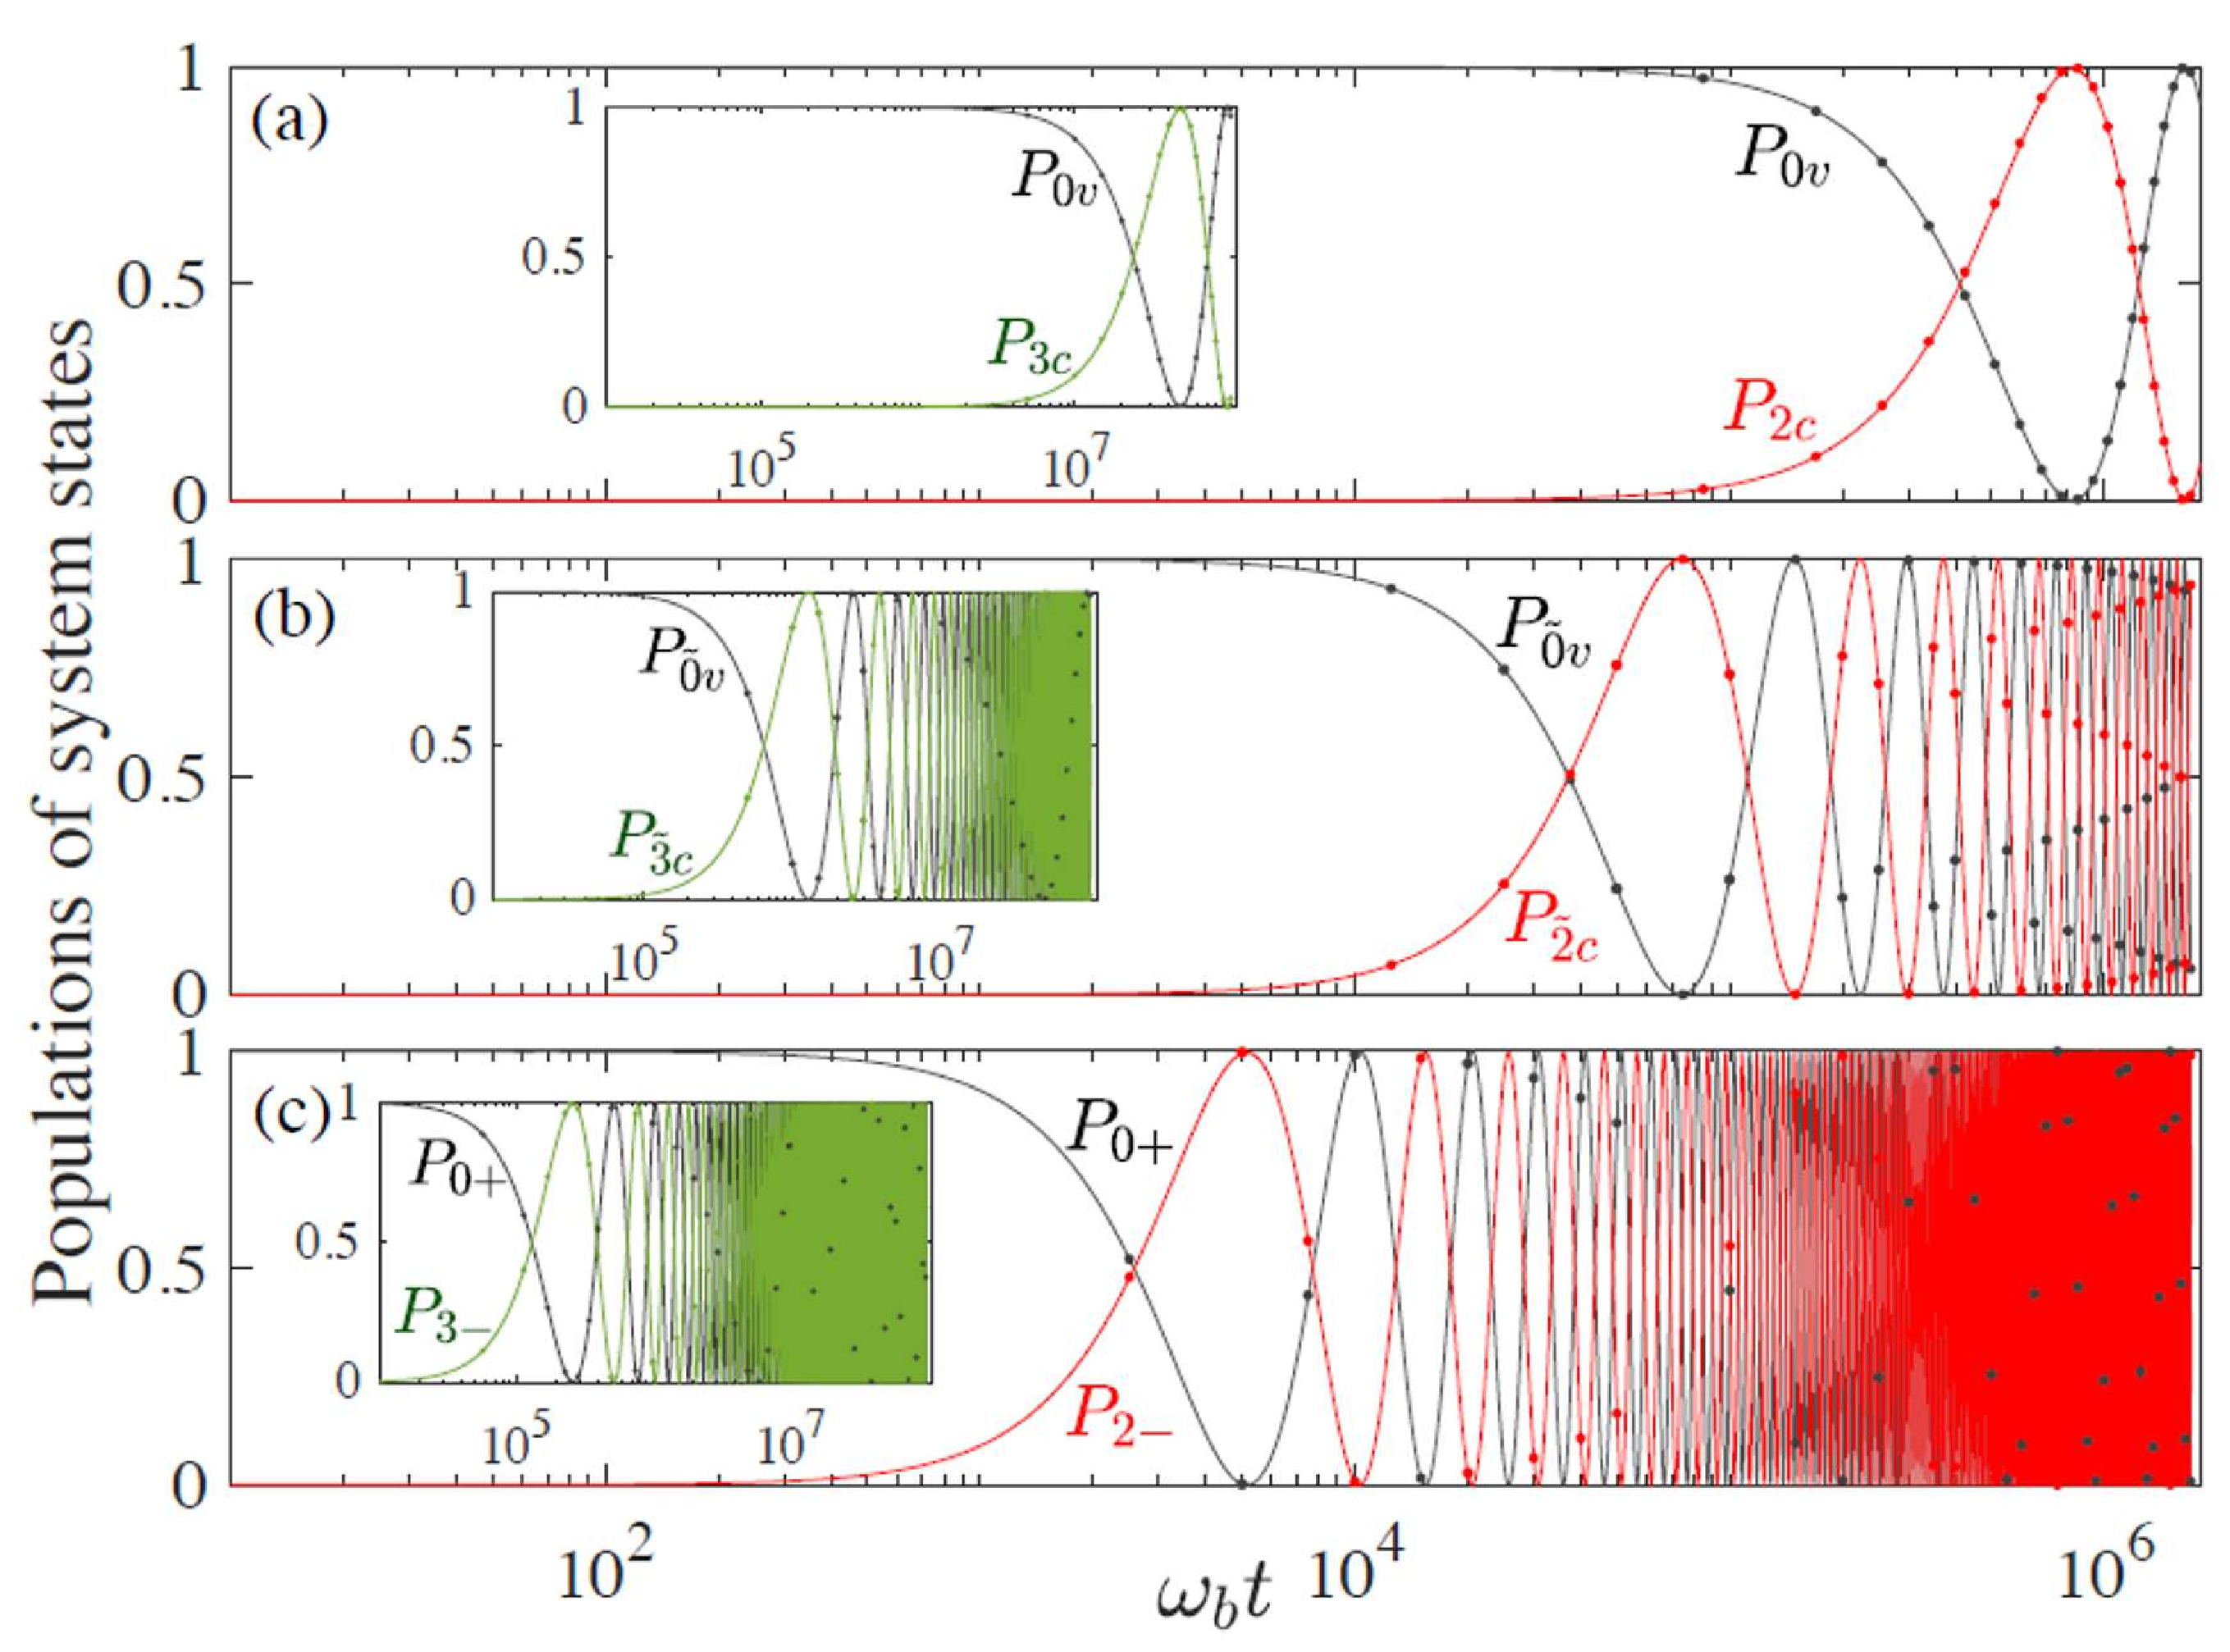
\includegraphics[width=0.7\linewidth]{img/super-Rabi}
	\caption{Oscilaciones gigante-Rabi vistas a través de la dinámica de la población $P_{jk}(t) = |\bra{j,k}\ket{\psi(t)}|^2\; (j=n,\tilde{n} \text{ y } k=c,v,+,-)$ con $n=2,3$ correspondiendo a la parte principal y recuadro, respectivamente \parencite{Bin2020}}
	\label{fig:super-rabi}
\end{figure}

Muestran que en los tres regímenes los estados 2- y 3-fonón son periodicamente generados, con alta fidelidad. Gracias a los procesos de Stokes. Este es el mecanismo básico para la generación de alta pureza de emisión bundle de $n$-fonón.

Comparando las figuras \ref{fig:super-rabi}(a), \ref{fig:super-rabi}(b) y \ref{fig:super-rabi}(c), se puede ver qué incrementando $\lambda$ y $\Omega$ aumenta la rapidez de las oscilaciones gigante-Rabi. Esto también se puede observar claramente desde las soluciones aproximadas analíticamente $\Omega_\text{eff}^{(n)}$ en todos los tres regímenes (ecuaciones \ref{eq:effRabi1}, \ref{eq:effRabi2} y \ref{eq:effRabi3}). Frecuencias más altas de oscilaciones conducen a tasas de emisión bundle $n$-fonón más altas.

\subsubsection{Dinámica del sistema abierto: emisión bundle $N$-fonón}
La disipación es el desencadenante de la emisión. Transfiere los estados $n$-fonón, mencionados anteriormente, dentro de la cavidad a bundles de $N$-fonones fuertemente correlacionados hacia afuera de la cavidad. Su fuerte correlación se puede ver por la función de correlación de fonones de igual-tiempo de $n$th-orden
\begin{equation}
	g^{(n)} = \frac{\braket{b^{\dagger n}b^n}}{\braket{b^\dagger b}^n}
\end{equation}

Para el primer régimen de parámetros la fig. \ref{fig:correlationbundle}(a) muestra las resonancias marcadas en la funciones de correlación (de abajo hacia arriba) de 2-orden, 3-orden, 4-orden y 5-orden. Claramente asociadas a las resonancias de Stokes $\Delta = -n\omega_b$. Se observa una caída dentro del pico bunching justo en la resonancia de 2-fonón en lugar de un pico de superbunching\footnote{Este término es usado para describir la estadística de partículas cuánticas. Se refiere a la tendencia, en un grado extremo, de las partículas a agruparse o emitirse juntas, por lo tanto, su correlación es muy fuerte.} (cómo se esperaría de una emisión multifonónica)\footnote{Aunque $g^{(n)}$ no garantice una actual emisión $n$-fonón, si debería revelar la intensidad de las correlaciones entre fonones y no lo hizo}. Sucede que el sistema entra en un nuevo régimen de emisión, a saber, bundles fuertemente correlacionados, en consecuencia,  para obtener la información completa del bundle se debe usar una función de correlación generalizada que describa al bundle como una cuasi-partícula

La funciones de correlación generalizadas $g_m^{(n)}$  son halladas sobre el bundle en sí mismo, es decir, como si fuese una nueva partícula y  da información sobre el bundle en sí mismo, es decir, si es antibunched (cañón de $n$-fonones), no correlacionado (láser de $n$-fonones) o bunched (estados térmicos de  bundles).

\begin{figure}[th]
	\centering
	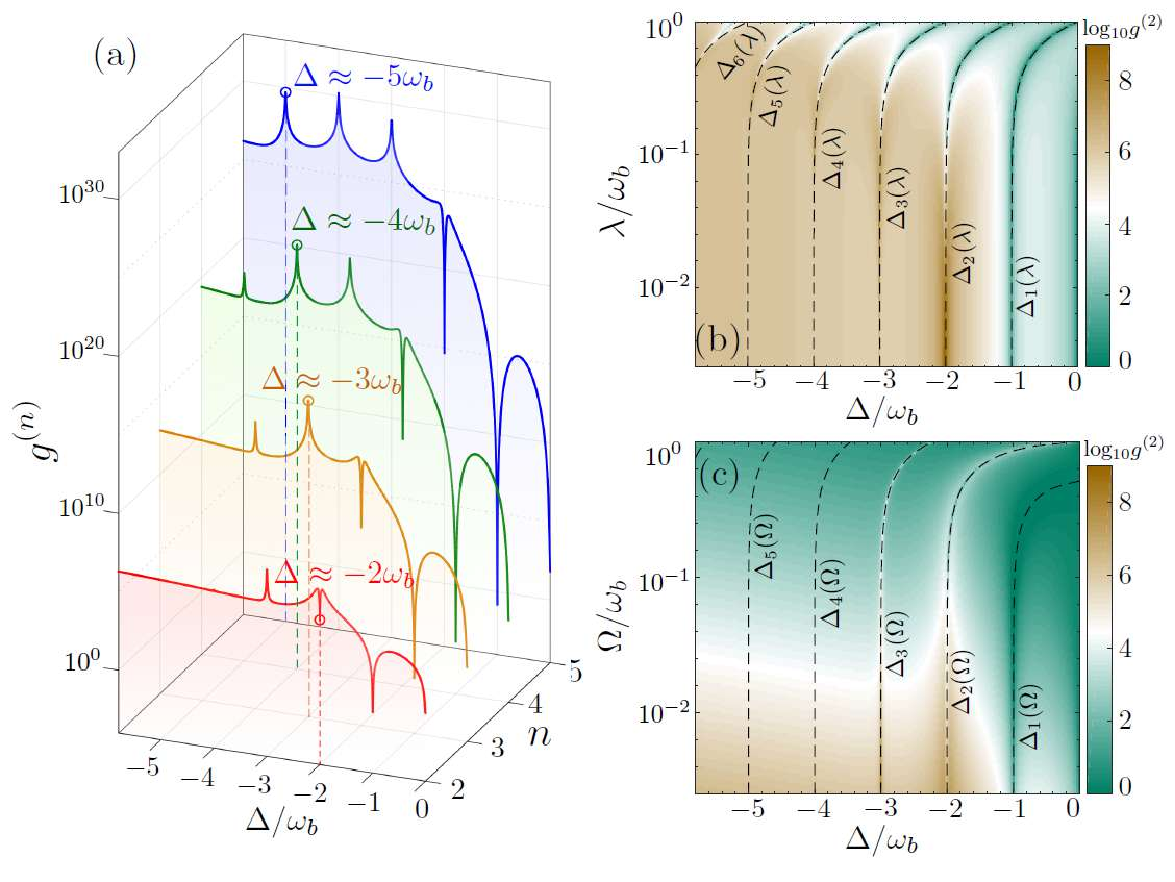
\includegraphics[width=0.8\linewidth]{img/correlationBundle}
	\caption{Funciones de correlación de $n$-th orden $g^{(n)}$ en igual-tiempo en función de $\Delta/\omega_b$. (b)-(c) Función de correlación $g^{(2)}$ para diferentes $\lambda/\omega_b$ (b) y $\Omega/\omega_b$ (c). Las líneas discontinuas indican las resonancias de $n$-fonones $\Delta=-n\omega_b$, $\Delta= \Delta_n(\lambda)$, y $\Delta = \Delta_n(\Omega)$. Los parámetros del sistema son (a) $\lambda/\omega_b= 0.03$, $\Omega/\omega_b = 0.003$, (b) $\Omega/\omega_b = 0.003$, (c) $\lambda/\omega_b = 0.03$, y  para los paneles (a)-(c) $\kappa/\omega_b = 0.002$, $\gamma/\omega_b = 0.0002$ y $\gamma_\phi/\omega_b = 0.0004$ \parencite{Bin2020}.}
	\label{fig:correlationbundle}
\end{figure}

Las figuras \ref{fig:correlationbundle}(b) y \ref{fig:correlationbundle}(c) muestran cómo al aumentar $\lambda$ y $\Omega$ las resonancias se desplazan (indicando el nuevo régimen). La figura muestra también que las diferencias de frecuencia de las resonancias $n$- $(n+1)$-fonón es casi independiente de $n$ (señal clara de resonancias de Stokes)

Para asegurar alta pureza de la emisión bundle $N$-fonón se debe suprimir las excitaciones fonónicas fuera de resonancia. Para ello se optimiza la frecuencia del bombeo de tal forma que $\omega_b \gg \kappa, \gamma$\footnote{Incluso para grandes $n$ \parencite{Bin2020}}. Con la técnica mencionada anteriormente se puede realizar una fuente versátil multi-fonónica controlada ópticamente, debido a que el orden $n$ del bundle puede ser controlado simplemente ajustando la frecuencia del bombeo láser.

Este tipo de fenómenos pueden ser importantes en el estudio de las interacciones cuánticas y la generación y manipulación de estados cuánticos de la luz y la materia, con posibles aplicaciones en tecnologías como la computación cuántica, las comunicaciones cuánticas y la sensibilidad cuántica.

%conclusiones
En conclusión, proponen un método eficiente para producir emisión bundle, de alta pureza\footnote{La emisión bundle con alta pureza ($>97\%$) se logró.}, de $n$-fonones basado en el proceso de Stokes, con bundles  fue obtenida sobre un amplio rango de parámetros. La pureza de la emisión $n$-fonón depende del decamiento de la cavidad y la intensidad del acoplamiento electrón-fonón, y es robusta con la intensidad del bombeo láser. La ventaja más destacada del método propuesto es la fácil sintonizción, simplemente ajustando la frecuencia del bombeo láser se pueden producir, esencialmente, emisiones puras de 2- y 3-fonones con la tecnología disponible actualmente.

%
\section[Oscilaciones gigante-Rabi de excitones oscuros sin campo magnético ...]{Oscilaciones gigante-Rabi de excitones oscuros sin campo magnético externo}\label{sec:giant-Rabi}
Los autores \parencite{Vargas2022} estudian un QD bombeado coherentemente con un láser externo. Considerando la base excitónica proporcionada por las diferentes alineaciones de espín del electrón y el hueco que componen el excitón. Inmerso en una cavidad acústica monomodal \parencite{Weib2018}. La base del QD se compone en total por 5 estados de matería: el base, 2 excitones brillantes y 2 excitones oscuros. Esta nueva base permite la descripción de interacciones más complejas en el sistema y posibilita el control de fenónemos interesantes.

Los principales aportes son: los excitones oscuros pueden ser excitados, aprovechando la interacción Beer-Pikus, ajustando finamente la frecuencia del láser\footnote{Sin la necesidad usual del campo magnético externo \parencite{Jimenez2017} lo cuál es más desafiante, y costoso, experimentalmente.}. Se pueden emitir bundles de $N$-fonones, ya que se puede realizar oscilaciones gigante-Rabi entre un estado vacío y un estado excitón oscuro $N$-fonón.

Entre las ventajas del método se destaca que el ajuste fino de la frecuencia del láser puede realizarse para apuntar a cualquier oscilación gigante-Rabi deseada para una amplia gama de parámetros, como las tasas de desintegración, las energías características y las constantes de acoplamiento. Lo destacado del método es que se puede pensar como una receta para generar oscilaciones gigante-Rabi. Lo cuál lo vuelve versátil para cualquier sistema, aunque La amortiguación de la oscilación depende de la naturaleza disipativa de la realización física del QD incrustado en una cavidad acústica.

Se considera un punto cuántico bombeado en una cavidad descrita por el siguiente Hamiltoniano \parencite{Bin2020}
\begin{equation}
	H = H_\text{QD} + H_\text{láser} + H_\text{cav} + H_\text{el-ph}
\end{equation}
ver ecuaciones \ref{eq:H_QD}, \ref{eq:5-laser}, \ref{eq:H_cav-ph} y \ref{eq:H_el-ph} para revisar con más detalle los términos que componen el sistema.

\subsubsection{Dinámica del sistema cerrado}
Hallan la dinámica del sistema sin interactuar con el entorno\footnote{Aunque no es una configuración realista del sistema, ayuda a comprender la física subyacente de la producción de oscilaciones gigante-Rabi}. Encuentran cómo y en qué estados se generan las oscilaciones gigante-Rabi. El acoplamiento electrón-fonón acompañado por el proceso de Stokes impulsado ópticamente a través del bombeo, permite la generación de oscilaciones gigante-Rabi entre los estados vacío $\ket{\text{phonons}=0}\otimes \ket{\text{QD}=v}$ (para débil bombeo láser ) y un estado propio del Hamiltoniano completo \parencite{Bin2020}. Se muestran las oscilaciones gigante-Rabi producidas seleccionando un estado propio compuesto principalmente de $N$ fonones y excitones oscuros (ver figura \ref{fig:eigenstatesgiant-rabi})

\begin{figure}[th]
	\centering
	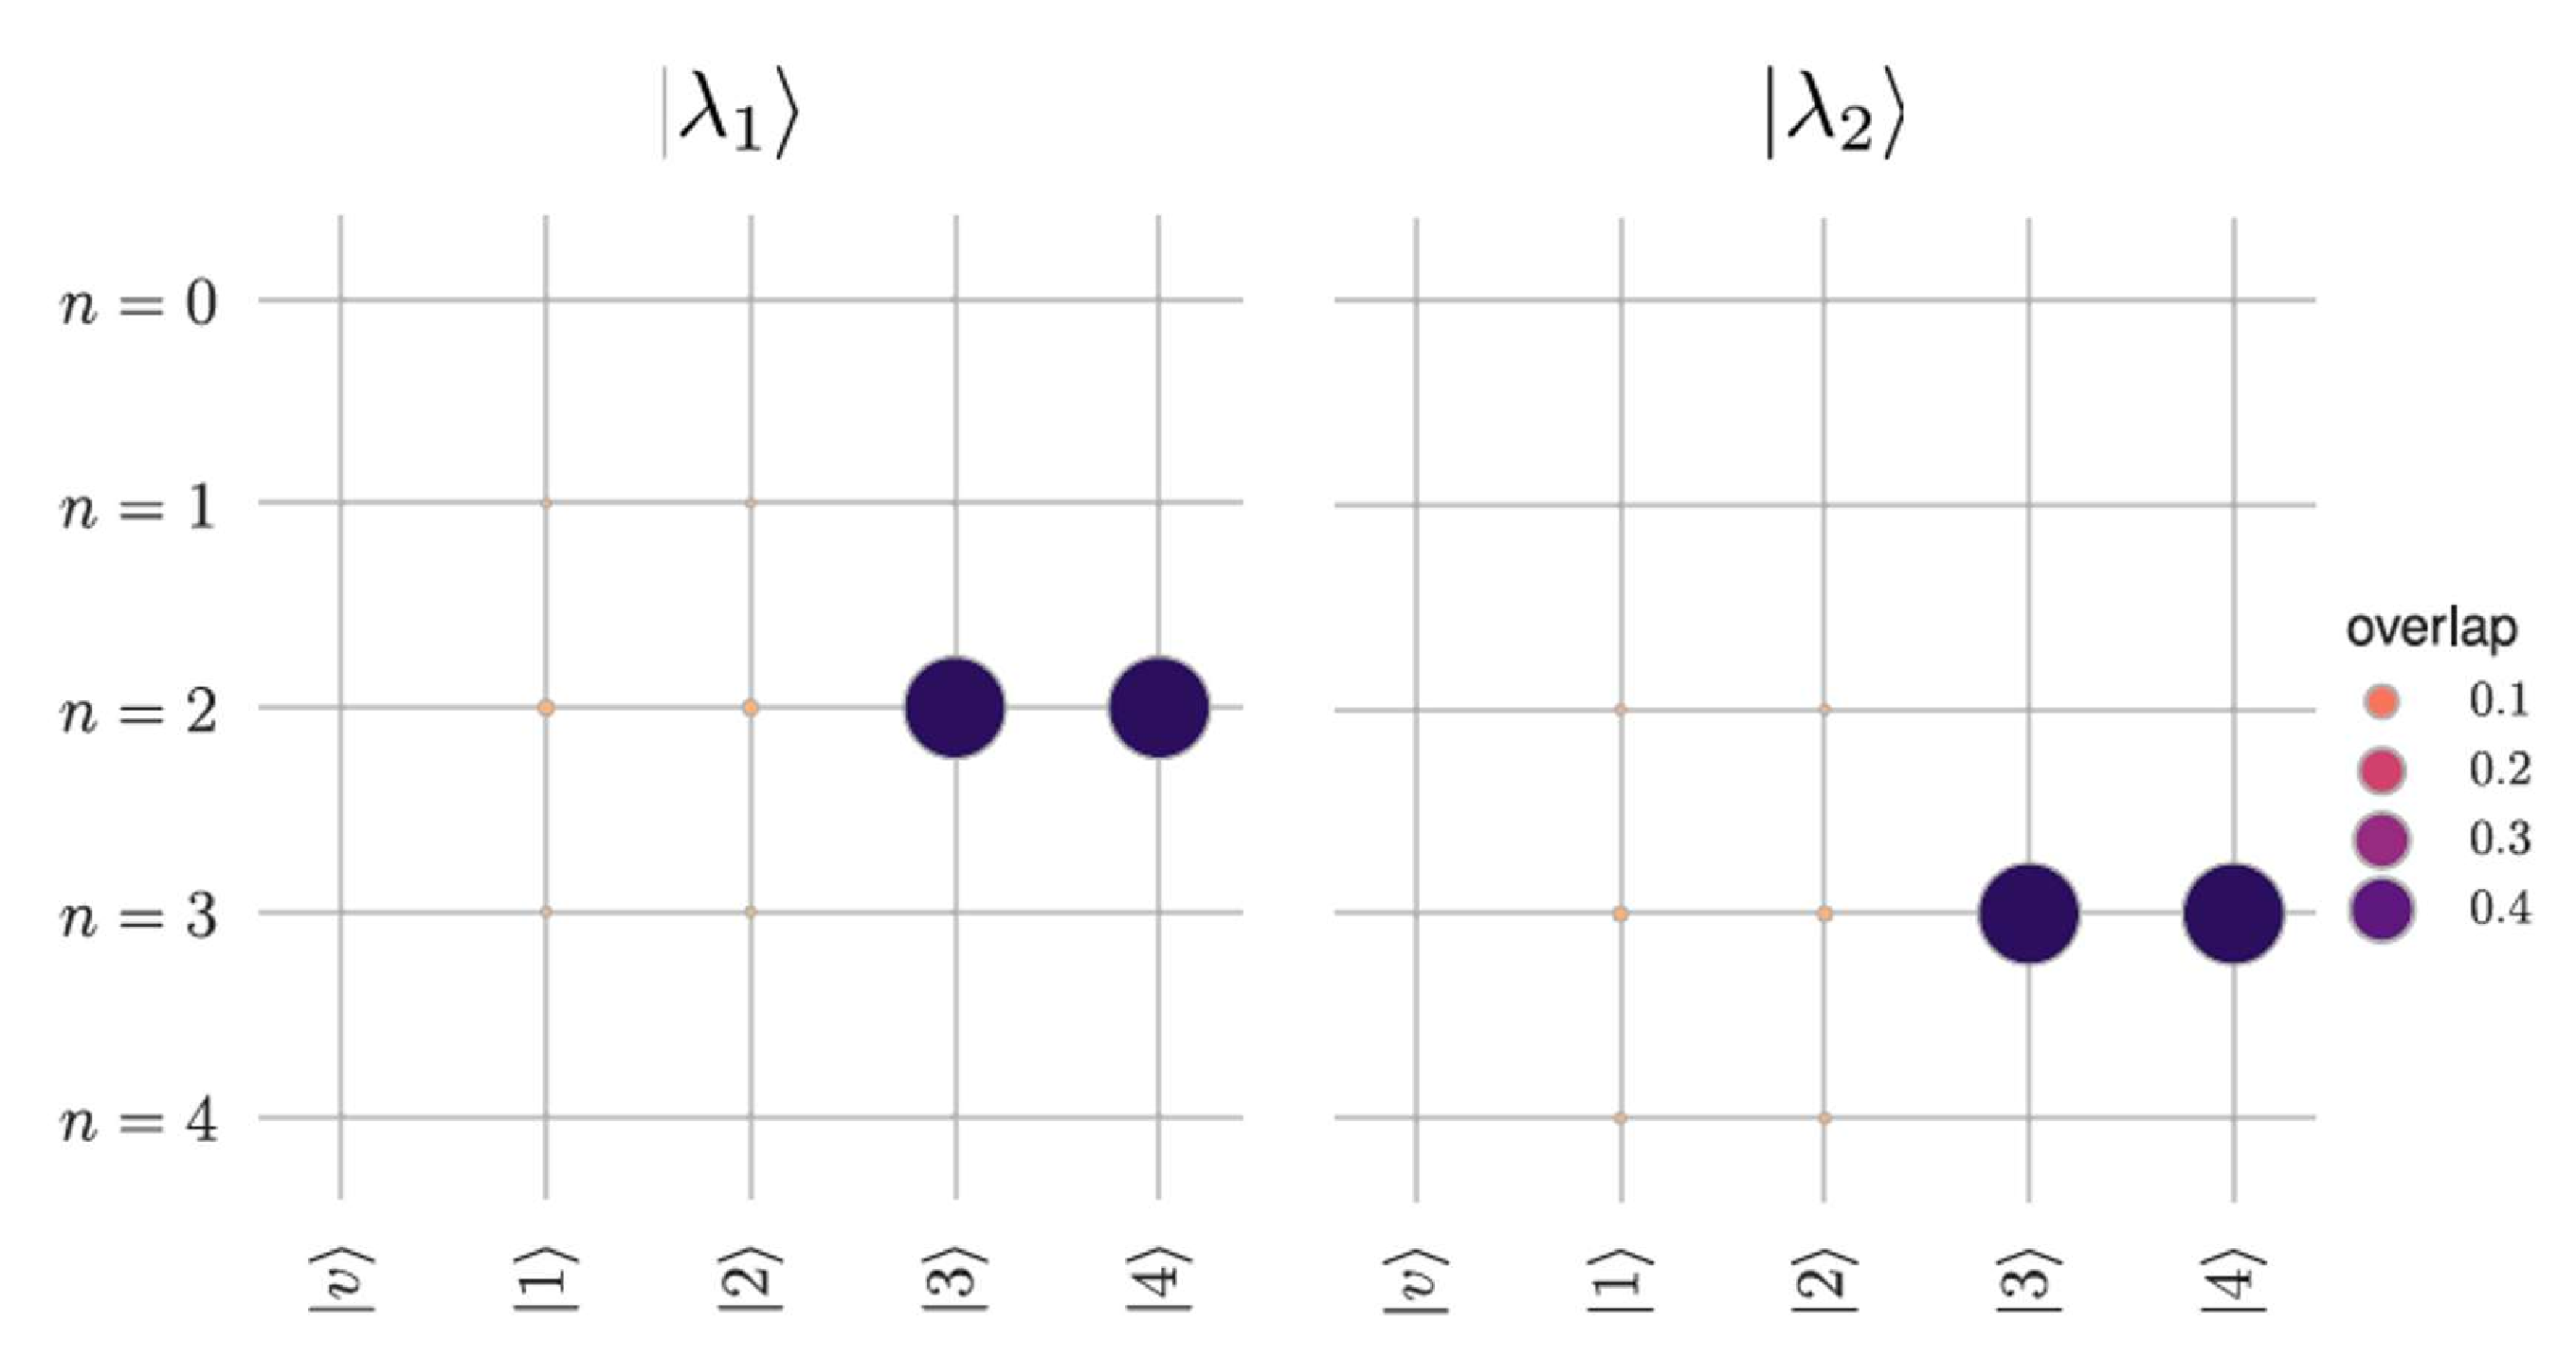
\includegraphics[width=0.75\linewidth]{img/EigenstatesGiant-Rabi}
	\caption{Estados propios del Hamiltoniano completo para acoplamiento débil electrón-fonón $(g= g_{bb} = g_{bd} \approx 0.02\omega_b)$, bombeando $(\Omega_1 \approx 0.082\omega_b,\, \Omega_2=0)$, y el láser externo en resonancia con la energía del brillante-excitón ($\omega_L=\omega_X$, donde la frecuencia del QD puede ser elegida para coincidir con cualquier energía excitón del QD semiconductor, e.g., $1.36$ eV para GaAs QDs). Estos valores se usan durante el paper excepto la frecuencia del láser que debe ser ajustada finamente \parencite{Vargas2022}.}
	\label{fig:eigenstatesgiant-rabi}
\end{figure}

El estado $\ket{*}\lambda_{1(2)}$ está compuesto en su mayoría por el estado $\ket{2(3),d_+}$, donde
\begin{equation}
	\ket{d_\pm} = \frac{\ket{3} \pm \ket{4}}{\sqrt{2}}
\end{equation}

Las oscilaciones gigante-Rabi se logran a través de un efecto cascada \parencite{Bin2020}, donde las transiciones del sistema van desde estado vacío $\ket{0,v}$ a un estado excitón brillante (dependiendo de las amplitudes del láser) y luego (mayoritariamente) a un estado simétrico excitón oscuro con $N$ fonones después de que el sistema sea guiado por el mecanismo de acoplamiento electrón-fonón.

\begin{figure}[th]
	\centering
	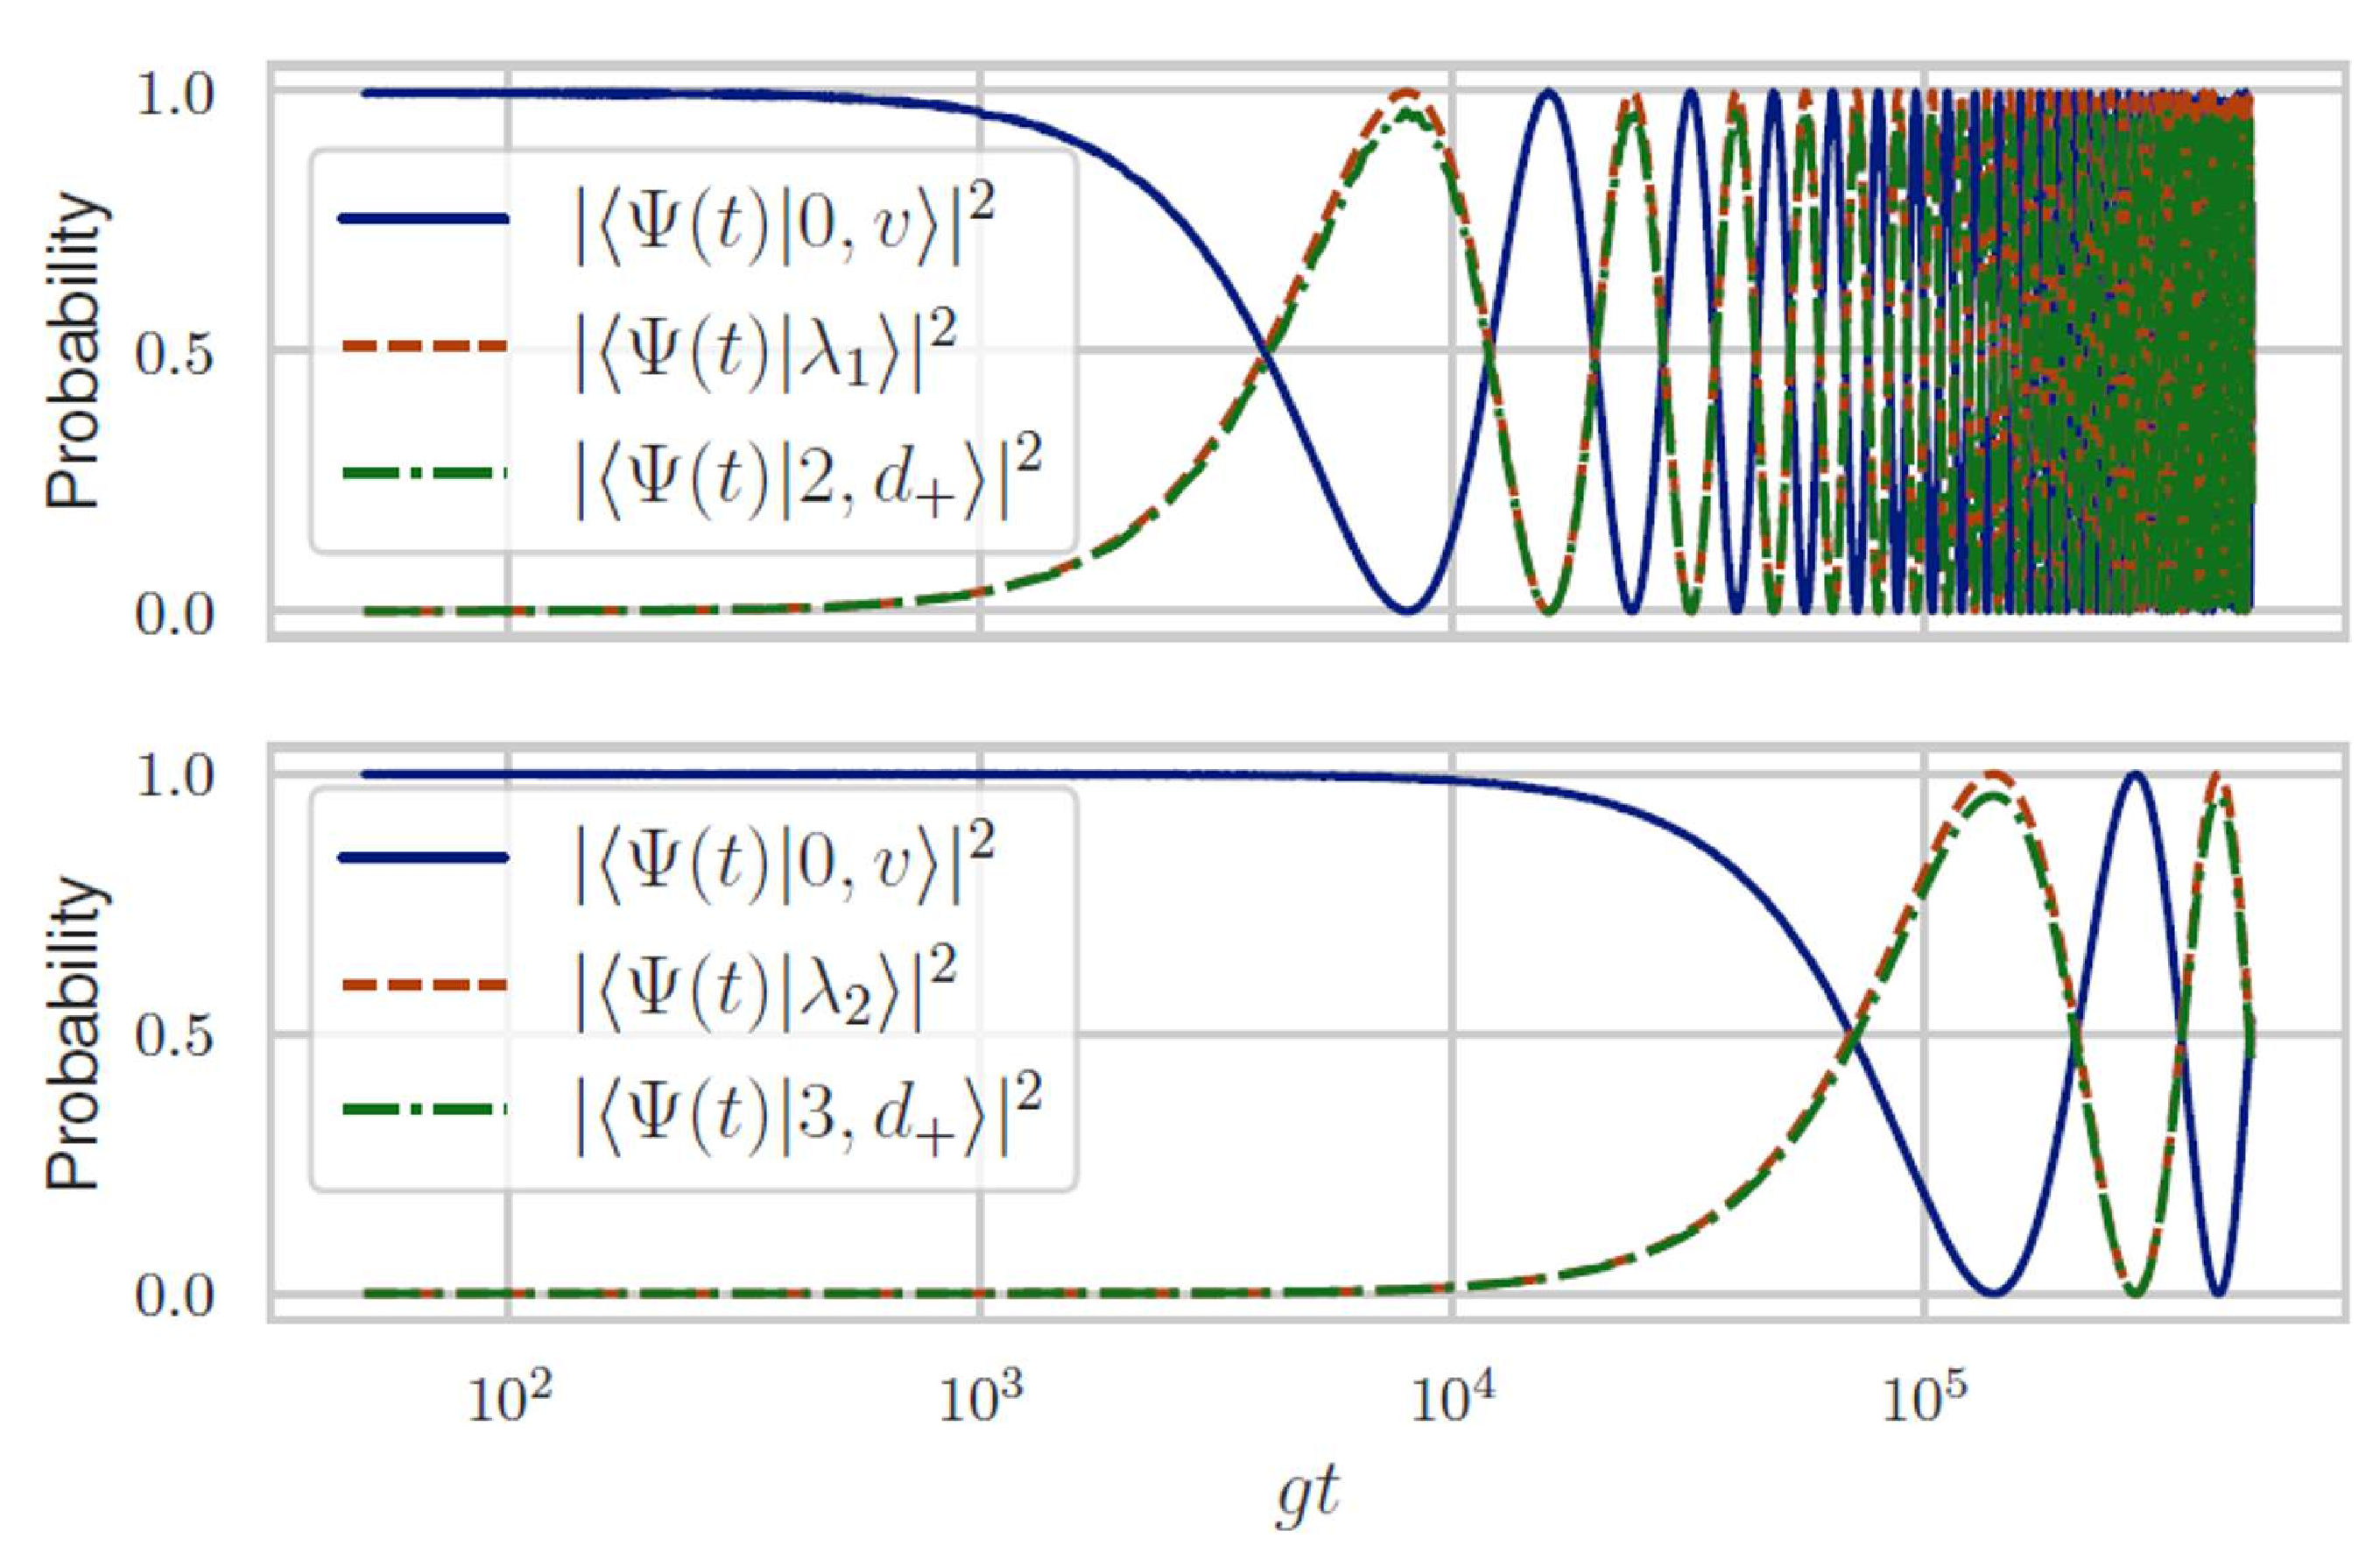
\includegraphics[width=0.7\linewidth]{img/EigenstatesGiant-Rabi1}
	\caption{Oscilaciones gigante-Rabi entre el estado de valencia de fonón $0$ (línea continua) y los estados mostrados en la fig. \ref{fig:eigenstatesgiant-rabi} (línea discontinua). La línea discontinua muestra la evolución del estado $\ket{n,d_+}$ para $n = 2$ (panel superior) y $n = 3$ (panel inferior). El desajuste del láser es $\Delta/\omega_b = (\omega_X-\omega_L)/\omega_b \approx 1.960$ para el panel superior, y $\approx 2.961$ para el panel inferior. Se utilizan las mismas condiciones de acoplamiento y bombeo de la fig. \ref{fig:eigenstatesgiant-rabi} \parencite{Vargas2022}.}
	\label{fig:eigenstatesgiant-rabi1}
\end{figure}

Muestran con ambos ejemplos que es posible ajustar la frecuencia del láser para apuntar a oscilaciones gigante-Rabi entre el vacío $\ket{0,v}$ y cualquier estado propio $\ket{\lambda}$ del Hamiltoniano completo, considerando una frecuencia láser
\begin{equation}
	\omega_L = \omega_\lambda - \omega_g
\end{equation}
donde $\omega_\lambda = \bra{\lambda}H\ket{\lambda}$ y $\omega_g$ es su frecuencia estado-base \parencite{Bin2020}. 

No se halló las oscilaciones gigante-Rabi para los estados $\ket{n,d_-}$ (estados de materia oscuro-excitón con antisimetría), aunque son eigenstates del Hamiltoniano completo, porque ellos no son accesibles de estados iniciales antisimétricos no oscuros, se puede comprobar con:
\begin{equation}
	\bra{m,\beta}H\ket{n,d_-} = 0
\end{equation}
donde $\ket{\beta}$ es cualquier estado abarcado por estados brillante-excitón, y $m$ es algún número de fonones. Se puede acceder a estos estados antisimétricos oscuro-excitón en la presencia de disipación.

\subsubsection{Dinámica del sistema abierto}
Para estudiar una configuración realista del sistema propuesto, es necesario hacer la descripción como un sistema abierto (ver ec. \ref{eq:dissipativeMasterEquation}). A través de los canales disipativos tal descripción muestra que las oscilaciones gigante-Rabi pueden emitir bundles de $N$-fonones (ver sección \ref{sec:StokesBundles}). 

\subsubsection{Espectro de emisión}
Para mostrar que los procesos de emisión $n$-fonón, con $n=2,3$, pueden ser resueltos en frecuencia se examina el espectro de emisión de fonones (véase la fig. \ref{fig:emissionspectrumgiant-rabi}(c)) por medio de la teoría espectral (ver sección \ref{sec:spectralTheory}).

El espectro de emisión de fonones $I(\omega)$ se puede obtener a través del teorema Wiener-Khintchine en analogía al espectro de fotoluminiscencia \parencite{Perea2004}
\begin{equation}
	I(\omega) \propto \frac{\kappa}{\pi} \int_0^\infty \braket{b(t) b^\dagger(t+\tau) e^{i\omega\tau}} d\tau
\end{equation}

\begin{figure}[th]
	\centering
	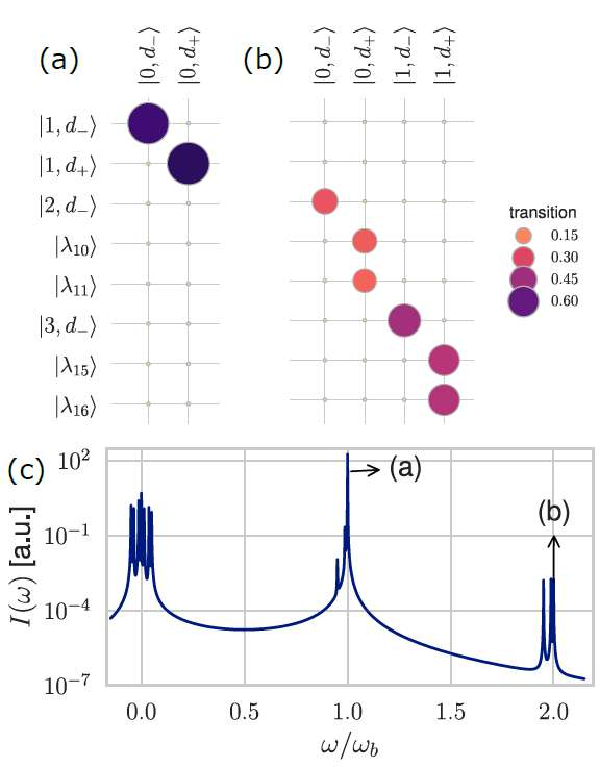
\includegraphics[width=0.55\linewidth]{img/emissionSpectrum_Giant-Rabi}
	\caption{Espectro de emisión de fonones $I(\omega)$. Los paneles (a) y (b) muestran los elementos $|\bra{\psi}\varrho\ket{\phi}|^2$ de las eigenmatrices Liouvillianas $\varrho$ que coinciden con los picos señalados en el espectro de emisión de fonones de la fig.\ref{fig:emissionspectrumgiant-rabi} \parencite{Vargas2022}.}
	\label{fig:emissionspectrumgiant-rabi}
\end{figure}


La figura \ref{fig:emissionspectrumgiant-rabi}(a) dice que  el pico más prominente del espectro coincide con las transiciones  entre estados oscuros con un fonón y estados oscuros con cero fonones\footnote{La excitación de las transiciones depende de la energía inyectada en el sistema y la intensidad de las interacciones que permiten ciertas transferencias de población.}. La figura \ref{fig:emissionspectrumgiant-rabi}(b) nos muestra las transiciones permitidas para otro pico a una frecuencia de $\omega = 2\omega_b$, que coincide con las transiciones entre estados oscuros con dos fonones decayendo a estados oscuros sin fonones, y también estados oscuros con tres fonones decayendo a estados oscuros con un fonón. 

Lo destacado del espectro de emisión es que el pico de emisión que coincide con 2-fonón es mucho más pequeño que el pico 1-fonón. Estas transiciones correspondientes pueden ser diferenciadas debido a la gran diferencia de energía en el espectro. Se asocia las frecuencias sideband con los picos del espectro de emisión fonónica debido a que se deben a transiciones entre estados oscuros y brillantes acompañadas de emisión de 0-, 1-, y 2-fonón, respectivamente.

%conclusiones
En conclusión, los excitones oscuros son más robustos a la decoherencia, porque ellos no pueden acoplarse a los modos ópticos de fuga, y pueden ser dirigidos para realizar oscilaciones gigante-Rabi entre estados oscuros con $N$ fonones y el vacío. Estas oscilaciones gigante-Rabi muestran un proceso en cascada restringido que acopla estados con diferente número de fonones, resultando finalmente en un acoplamiento efectivo entre el vacío y un estado excitón-oscuro-simétrico con $N$ fonones. Cuando se abren los canales disipativos, otros estados intermedios son activados en el proceso en cascada, culminando en la emisión bundle de $N$-fonón. Para los parámetros estudiados, las funciones de correlación del bundle de $N$-fonón muestran estadísticas cuánticas correspondientes a antibunching\footnote{Propiedad deseada para realizar cañones $N$-fonón.}. A través del análisis del espectro de emisión, caracterizan las transiciones acústicas del sistema, demostrando que la emisión bundle de $N$-fonón puede ser resuelta en frecuencia\footnote{Característica importante para distinguir experimentalmente las cuasipartículas de fonones que escapan de la cavidad acústica.}.

%
\section{Estructura fina de excitones neutros y cargados en puntos cuánticos In(Ga)As / (Al)GaAs autoensamblados}

Los autores \parencite{Bayer2002} realizan un estudio sobre la estructura fina de los puntos cuánticos neutros y cargados de  In(Ga)As/(Al)GaAs. En este estudio, se han realizado experimentos y análisis teóricos para entender la estructura fina de estos puntos cuánticos. El documento menciona experimentos que implican la medición de las energías de transición de excitones en diferentes puntos cuánticos en función del campo magnético. Los excitones son pares de electrones y huecos que se atraen mutuamente y pueden existir en semiconductores y aislantes. De los resultados experimentales del estudio se establecen los parámetros para la simulación. Los valores usados son típicos para QDs auto ensamblados InAs/GaAs bajo un campo magnético: $\delta_0 = 0.2 \text{ meV}, \, \delta_1 = 0.18 \text{ meV},\, \delta_2 = 0.05 \text{meV},\, g_{hx} = -0.35,\, g_{hz} = -2.2,\, g_{ex} = -0.65,\, g_{ez} = -0.8$.
\end{document}